\documentclass{scrartcl}
\usepackage[T1]{fontenc} 
\usepackage{lmodern}
\usepackage{booktabs}
\usepackage{hyperref}
\usepackage[margin=2cm]{geometry}
\usepackage{listings}
\usepackage{xcolor}
\usepackage{nicefrac}
\usepackage{graphicx}
\usepackage{fontspec}
\usepackage{tikz}
\usepackage{microtype}
\usepackage{float}
\usepackage{amsmath}
\restylefloat{table}

\definecolor{gruvbox-black}{RGB}{40, 40, 40}
\definecolor{gruvbox-red}{RGB}{204, 36, 29}
\definecolor{gruvbox-green}{RGB}{152, 151, 26}
\definecolor{gruvbox-gray}{RGB}{168, 153, 132}
\definecolor{gruvbox-darkgray}{RGB}{146, 131, 116}
\definecolor{gruvbox-beige}{RGB}{235, 219, 178}
\definecolor{gruvbox-brightbeige}{RGB}{251, 241, 199}

\usepackage{plex-serif}
\usepackage{plex-sans}
\setmonofont{input-mono}

\pagecolor{gruvbox-black}
\color{gruvbox-brightbeige}

\definecolor{dkgreen}{rgb}{0,0.6,0}
\definecolor{gray}{rgb}{0.5,0.5,0.5}
\definecolor{mauve}{rgb}{0.58,0,0.82}

\lstset{frame=tb,
  language=Python,
  aboveskip=3mm,
  belowskip=3mm,
  showstringspaces=false,
  columns=flexible,
  basicstyle={\small\ttfamily\color{gruvbox-beige}},
  numbers=none,
  numberstyle=\tiny\color{gruvbox-gray},
  keywordstyle=\color{gruvbox-red},
  commentstyle=\color{gruvbox-darkgray},
  stringstyle=\color{gruvbox-green},
  breaklines=true,
  breakatwhitespace=true,
  tabsize=3
}


\setlength{\parindent}{10pt}
\setlength{\parskip}{1ex plus 0.5ex minus 0.5ex}

\begin{document}
\begin{center}{\textbf{\LARGE Advanced HD Video Encoding Guide} \\[3mm]
Not everything is going to be 100\% correct and certain parts are missing.
\url{https://git.concertos.live/Encode_Guide/Encode_Guide/}}
\end{center}

\vspace{50pt}
\tableofcontents
\pagebreak

\section{Tools}

\subsection{eac3to}

While we don't like to recommend closed source software, there's no denying that \texttt{eac3to} \footnote{\url{https://forum.doom9.org/showthread.php?t=125966}} is a very useful tool for the demuxing process with no really good alternatives.  If you don't want to download closed source software (let alone support it), you can also simply use MKVToolNix \footnote{\url{https://mkvtoolnix.download/}} without a separate demuxer.

For Windows users, simply download this from Doom9.  Unix users will have to use Wine.  When specifying the path, either use Winepath or swap out the slashes accordingly yourself.

\subsection{VapourSynth}

VapourSynth's installation is simple.  There's an installer for Windows, Homebrew for Mac, and every distro's repository should have VapourSynth.

The VapourSynth documentation lists paths for where to place your plugins.  The recommended path for Windows is \texttt{<AppData>\textbackslash VapourSynth\textbackslash plugins32} or\\ \texttt{<AppData>\textbackslash VapourSynth\textbackslash plugins64}.  Unix users can create a configuration file to specify paths.

Python scripts for VapourSynth should be placed in your Python \texttt{site-packages} folder.  On Arch Linux, this is \texttt{/usr/lib64/Python3.*/sitepackages/}.  Windows users will find this in their local AppData folder.

\subsection{Editors}

There are four popular editors for VapourSynth:
\begin{itemize}
\item VapourSynth Editor\footnote{\url{https://bitbucket.org/mystery_keeper/vapoursynth-editor}}
\item Yuuno\footnote{\url{https://yuuno.encode.moe}}
\item VapourSynth Preview\footnote{\url{https://github.com/Endilll/vapoursynth-preview/}}
\item AvsPmod\footnote{\url{https://avspmod.github.io/}}
\end{itemize}

Every Linux repository should have VSEdit.  In Arch, for example, it's in \texttt{aur/vapoursynth-editor}.  There's an installer for Windows, and Mac users should be able to install it via Homebrew.

Yuuno is an extension for Jupyter notebooks that allows you to edit and export VapourSynth scripts.  You can install it via \texttt{\$ pip install yuuno} and then \texttt{\$ yuuno jupyter install}.  Note that you'll need to have Jupyter or Jupyter Lab installed.

VapourSynth Preview requires a separate text editor or IDE to write the scripts, which makes it very useful for those who don't like the editor included in VSEdit.

AvsPmod is the editor used for AviSynth, but it also supports VapourSynth.

They all have their advantages and disadvantages, but for new users, I'd recommend VSEdit for local editing and yuuno for users looking to also write their scripts on servers.  This is because Jupyter requires very little tinkering to work remotely.  One tip for yuuno users would be to try out Jupyter Lab as a replacement for Jupyter.

Here are the most important differences between these two:\\
\textbf{VSEdit}
\begin{itemize}
\item Doesn't require having your browser open.
\item Built-in benchmarking and encoding tools.
\item Easy skimming through video via CTRL + SHIFT + ARROW KEYS.
\item More stable.
\item Barely under development anymore.
\item Most private tracker users use this, hence it might be easier to get support.
\item VapourSynth-specific syntax highlighting and suggestions.
\item Allows you to store snippets and templates.
\end{itemize}
\textbf{yuuno}
\begin{itemize}
\item Very easy to use remotely.
\item Easy exporting via iPython magic.
\item Way better comparison tools via \texttt{\%\%vspreview clipa -{}-diff clipb} $\Rightarrow$ hovering over preview changes clip.
\item Less mature and hence more prone to breaking.
\item Allows you to work on and export multiple scripts from within one Jupyter Notebook.
\end{itemize}

\subsection{x264 and x265}

When installing x264 and x265, which are even easier to find than VapourSynth, you can also go with some mods.  The most popular mod for x264 is tmod.  Note worthy changes include \texttt{fade-compensate}, which can help encode fades with \texttt{mbtree} on, and more aq modes.  Unless you're using one of these options, which almost nobody does, you can just use vanilla x264 instead.  If you want to be even more precise when encoding, you can certainly give this a try and chain aq modes, since you might be able to squeeze a bit higher aq out of one of them to preserve dither while not ruining lines.

The most popular x265 mod, yukki, is even less impressive.  All this includes is some cosmetic changes like a nicer ETA.

\subsection{Opus, qAAC, and fdkaac}

For encoding Opus, you need the \texttt{opus-tools} package.

qAAC requires iTunes libraries.  On a Mac, this is no issue.  Windows users can install iTunes or QuickTime.  An alternative to this is the portable installer, which includes the necessary libraries with no iTunes requirements.  Arch users can use the \texttt{qaac-wine} package from the AUR.

If you want to use fdkaac instead, this is a simple install everywhere.

\subsection{MKVToolNix}

Install the latest mkvtoolnix.  This will install multiple tools, with the most important ones being \texttt{mkvtoolnix-gui} and \texttt{mkvextract}.

\section{Demuxing}

%\subsection{eac3to Usage}
%
%From my experience, Unix users just have to use Windows paths (or \texttt{winepath}).  From there, it's simply the following commands (and a few super similar ones) that may be of interest:
%\begin{align*}
%&\texttt{\$ wine eac3to.exe "\textbackslash path\textbackslash to\textbackslash source\textbackslash" -demux -progressnumbers}
%\\
%&\texttt{\$ wine eac3to.exe "\textbackslash path\textbackslash to\textbackslash source\textbackslash" 1:video.h264}
%\\
%&\texttt{\$ wine eac3to.exe "\textbackslash path\textbackslash to\textbackslash source\textbackslash" 2:audio\_core.ac3 -core}
%\\
%&\texttt{\$ wine eac3to.exe "\textbackslash path\textbackslash to\textbackslash source\textbackslash" 2:audio\_lossless.wav}
%\\
%&\texttt{\$ wine eac3to.exe "\textbackslash path\textbackslash to\textbackslash source\textbackslash" -changeto24.000 -23.976}
%\end{align*}
%
%You shouldn't use it to convert to lossy formats, as its encoders suck.  Just use it to extract stuff.

\subsection{ffmpeg and bdinfo}

For demuxing, there's a fantastic wrapper around \texttt{ffmpeg} called \texttt{bdinfo}\footnote{\url{https://github.com/schnusch/bdinfo}}.  Despite sharing its name with the other BDInfo program, it can't produce the same scans which many sites require.  The README on the GitHub repository should suffice for use.  You'll mainly need the \texttt{-x} and \texttt{-L} options.

\subsection{50\,fps, HEVC Seamless Branching, and Other eac3to Problems}

If you encounter a Blu-ray with seamless branching (i.e.\ your playlists consist of hundreds of \texttt{m2ts} files played after each other) with HEVC streams, you'll have to use \texttt{makemkv} instead.

Other issues with \texttt{ffmpeg} and \texttt{bdinfo} (the errors are actually with \texttt{libbluray}) may also be solved by using \texttt{makemkv} or directly plugging the source into \texttt{mkvtoolnix}.

\section{Video Encoding}

\subsection{Your First Script}

A standard VapourSynth super basic script with no extra filtering done will look something like this:
\begin{lstlisting}
# Uncomment the following line if you're using yuuno as apposed to VSEdit:
#%load_ext yuuno # This tells Jupyter to load yuuno.
#%%vspreview # This will allow you to preview the output.

# This section is for VSEdit #
import vapoursynth as vs
core = vs.core
##############################

src = core.ffms2.Source("/path/to/source.mkv") # For Windows paths, use r"C:\path\to\source.mkv".
out = core.std.Crop(src, top=138, bottom=138) # Crop off black bars as necessary.

out.set_output() # flags the variable as the output for vspipe
\end{lstlisting}

\subsubsection{Resizing}

% TODO: mention ewa_lanczos via placebo.resample

Firstly, note that there'll be a separate section later on for descaling.  Here, I'll explain resizing and what resizers are good for what.

If you want to resize, it's important to not alter the aspect ratio more than necessary.  If you're downscaling, first figure out what the width and height should be.  If you want to downscale to 720p, first crop, then figure out whether you're scaling to 720 height or 1280 width.  If the former is the case, your width should be:
\begin{lstlisting}
width = round(720 * src.height / (2 * src.width)) * 2
\end{lstlisting}
For the latter, the code to find your height is quite similar:
\begin{lstlisting}
height = round(1280 * src.width / (2 * src.height)) * 2
\end{lstlisting}

You can also use the \texttt{cropresize} wrapper in \texttt{awsmfunc}\footnote{\url{https://git.concertos.live/AHD/awsmfunc/}} to do these calculations and resize.

There are many resizers available.  The most important ones are:
\begin{itemize}
\item \textbf{Point} also known as nearest neighbor resizing, is the simplest resizer, as it doesn't really do anything other than enlargen each pixel or create the average of surrounding each pixel when downscaling.  It produces awful results, but doesn't do any blurring when upscaling, hence it's very good for zooming in to check what each pixel's value is.  It is also self-inverse, so you can scale up and then back down with it and get the same result you started with.
\item \textbf{Bilinear} resizing is very fast, but leads to very blurry results with noticeable aliasing.
\item \textbf{Bicubic} resizing is similarly fast, but also leads to quite blurry results with noticeable aliasing.  You can modify parameters here for sharper results, but this will lead to even more aliasing.
\item \textbf{Lanczos} resizing is slower and gets you very sharp results.  However, it creates very noticeable ringing artifacts.
\item \textbf{Blackmanminlobe} resizing, which you need to use \texttt{fmtconv}\footnote{\url{https://github.com/EleonoreMizo/fmtconv/}} for, is a modified lanczos resizer with less ringing artifacts.   This resizer is definitely worth considering for upscaling chroma for YUV444 encodes (more on this later).
\item \textbf{Spline} resizing is quite slow, but gets you very nice results.  There are multiple spline resizers available, with \texttt{Spline16} being faster than \texttt{Spline36} with slightly worse results, and \texttt{Spline36} being similar enough to \texttt{Spline64} that there's no reason to use the latter.  \texttt{Spline36} is the recommended resizer for downscaling content.
\item \textbf{nnedi3}\footnote{\url{https://gist.github.com/4re/342624c9e1a144a696c6}} resizing is quite slow and can only upscale by powers of 2.  It can then be combined with \texttt{Spline36} to scale down to the desired resolution.  Results are significantly better than the aforementioned kernels.
\item \textbf{FSRCNNX}\footnote{\url{https://github.com/igv/FSRCNN-TensorFlow/releases}} is a shader for mpv, which can be used via the \texttt{vs-placebo}\footnote{\url{https://github.com/Lypheo/vs-placebo}} plugin.  It provides far sharper results than \texttt{nnedi3}, but requires a GPU.  It's recommended to use this for upscaling if you can.
\end{itemize}
A comparison of these resizers can be found in the appendix under figure \ref{fig:14} for downscaling and figure \ref{fig:15} for upscaling.  Additionally, as changing its parameters will have a very significant result on the output, a comparison of differently configured bicubic upscales is included after these in figure \ref{fig:22}.  For the extra curious, I've included a comparison of downscales scaled back to the original resolution in figure \ref{fig:20}, as well as one showcasing the same resizer for downscaling then upscaling in figure \ref{fig:21} in the appendix.

While these screenshots should help you get a decent idea of the differences between resizers, they're only small parts of single images.  If you want to get a better idea of how these resizers look, I recommend doing these upscales yourself, watching them in motion, and interleaving them (\texttt{std.Interleave}).

The difference between resizers when downscaling is a lot less noticeable than when upscaling.  However, it's not recommended to use this as an excuse to be lazy with your choice of a resize kernel when downscaling.

TL;DR: Use \texttt{core.resize.Spline36} for downscaling.

\pagebreak

\subsection{Filtering}

There are a few things worth mentioning here.  First of all, most Blu-rays come in YUV420P8 with limited range.  The first group of information here is YUV.  This stands for the planes our video has, with Y being luma and U and V being our chroma planes.  

The color after that, 4:2:0 in this case, specifies the size of our planes.  The three most common variations of this are 4:2:0, which means that chroma planes are half the size of the luma plane (e.\@g.\ a $1920\times1080$ video will have chroma planes in $960\times540$), 4:2:2, which means that the chroma planes are half the size on their horizontal axis and full size on the vertical axis, and 4:4:4, which means all planes are the same size.  During playback, video players scale the chroma planes up to the same size as the luma.  Smaller chroma planes aren't as noticeable, but one can certainly tell the difference when upscaling.  To illustrate this, here's an example from AnoHana with one image being 4:2:0 720p upscaled to 1080p and the other being 4:4:4 720p upscaled to 1080p:

\begin{figure}[h]
\begin{minipage}{.5\textwidth}
\centering
\includegraphics{Pictures/yuv420.png}
\end{minipage}
\begin{minipage}{.5\textwidth}
\centering
\includegraphics{Pictures/yuv444.png}
\end{minipage}
\caption{YUV420 on left, YUV444 on right.  Descaled with \texttt{fvf.Debicubic}, then upscaled with \texttt{nnedi3\_rpow2.nnedi3\_rpow2} and \texttt{resize.Bilinear}.  Zoomed in with a factor of 2.}\label{fig:11}
\end{figure}

In this case, the worst resizer (bilinear) was used for the chroma planes.  If you use something like mpv with KrigBilateral, this should look far better.

Another example: the Parasite SDR UHD in 4:4:4 1080p compared to 4:2:0 1080p:
\begin{figure}[h]
\centering
\includegraphics{Pictures/yuv420vsyuv444.png}
\caption{Parasite SDR UHD scaled to 1080p 4:2:0 compared to 4:4:4.  Thanks go out to HyerrDoktyer for this example.}
\end{figure}

The next piece of information to explain is P8.  This refers to the bit depth, which is 8-bit in this case.  Most video is stored in 8-bit nowadays, as 8-bit AVC has the best hardware compatibility.  However, as 8-bit leads to not having enough values (0-255) available, it easily introduces errors such as banding.  Higher bit depths don't have such big issues with this, and due to their better accuracy, some (i.\@e.\ 10-bit) are actually better at storing video at lower file sizes.  However, 10-bit AVC has almost no hardware compatibility and takes a lot longer to encode, hence people on private trackers usually dislike it.  Most content is actually produced in either 10-bit or 12-bit.  The most popular bit depth for filtering is 16-bit due to increased accuracy.  It's worth noting that UHD Blu-rays will be in YUV420P10, meaning 10-bit.

The final piece to the puzzle here is limited range.  In full range 8-bit, we have every value between 0 and 255 available.  However, TVs usually can't display all these values and are limited to a range of 16 to 235 for luma and 16 to 240 for chroma.  Lots of consumer content, e\@.g.\ Blu-rays are also in limited range.  If you give a TV a full range video, it will simply make everything 16 and under or 235/240 and over the same value (e.g.\ black or white).

\subsubsection{Checking Your Source}
This is what will probably take up the most time: checking your source for issues.  This requires going through your entire source file and checking with your own eyes for banding, aliasing, dirty lines, and whatever other issues might be present.  The good news is that VSEdit allows you to simply go through your source by a self defined step via the CTRL + SHIFT + LEFT/RIGHT ARROW keys.  This step can be defined in the bottom right hand corner of the preview window.  I'd recommend a step between 1\,s and 3\,s.  Obviously, the slower the better, since you'll be covering more frames.

In order to apply a filter to a given range, use something like the following:
\begin{lstlisting}
filtered = my_filter(src)
out = awf.rfs(src, filtered, mappings="[FIRST_FRAME LAST_FRAME]")
\end{lstlisting}

\subsubsection{Dithering}

Although not necessary to work in if you're exporting in the same bit depth as your source, working in high bit depth and dithering down at the end of your filter chain is recommended in order to avoid rounding errors, which can lead to artifacts such as banding (an example is in figure \ref{fig:flvls}).  Luckily, if you choose not to write your script in high bit depth, most plugins will work in high bit depth internally.  As dithering is quite fast and higher depths do lead to better precision, there's usually no reason not to work in higher bit depths other than some functions written for 8-bit being slightly slower.

If you'd like to learn more about dithering, the Wikipedia page\footnote{\url{https://en.wikipedia.org/wiki/Dither}} is quite informative.  There are also a lot of research publications worth reading.  What you need to understand here is that your dither method only matters if there's an actual difference between your source and the filtering you perform.  As dither is an alternative of sorts to rounding to different bit depths, only offsets from actual integers will have differences.  Some algorithms might be better at different things from others, hence it can be worth it to go with non-standard algorithms.  For example, if you want to deband something and export it in 8-bit but are having issues with compressing it properly, you might want to consider ordered dithering, as it's known to perform slightly better in this case (although it doesn't look as nice).  To do this, use the following code:
\begin{lstlisting}
source_16 = fvf.Depth(src, 16)

deband = core.f3kdb.Deband(source_16, output_depth=16)

out = fvf.Depth(deband, 8, dither='ordered')
\end{lstlisting}
Again, this will only affect the actual debanded area.  This isn't really recommended most of the time, as ordered dither is rather unsightly, but it's certainly worth considering if you're having trouble compressing a debanded area.  You should obviously be masking and adjusting your debander's parameters, but more on that later.

In order to dither up or down, you can use the \texttt{Depth} function within either \texttt{fvsfunc}\footnote{\url{https://github.com/Irrational-Encoding-Wizardry/fvsfunc}} (fvf) or \texttt{mvsfunc}\footnote{\url{https://github.com/HomeOfVapourSynthEvolution/mvsfunc/}} (mvf).  The difference between these two is that fvf uses internal resizers, while mvf uses internal whenever possible, but also supports \texttt{fmtconv}, which is slower but has more dither (and resize) options.  Both feature the standard Filter Lite error\_diffusion dither type, however, so if you just roll with the defaults, I'd recommend fvf.  To illustrate the difference between good and bad dither, some examples are included in the appendix under figure \ref{fig:12}.  Do note you may have to zoom in quite far to spot the difference.  Some PDF viewers may also incorrectly output the image.

I'd recommend going with Filter Lite (fvf's default or \texttt{mvf.Depth(dither=3)}, also the default) most of the time.  Others like Ostromoukhov (\texttt{mvf.Depth(dither=7)}), void and cluster (\texttt{fmtc.bitdepth(dither=8)}), standard Bayer ordered (\texttt{fvf.Depth(dither='ordered')} or \texttt{mvf.Depth(dither=0)}) can also be useful sometimes.  Filter Lite will usually be fine, though.

\subsubsection{Debanding}

% TODO: mention libplacebo.Deband

This is the most common issue one will encounter.  Banding happens when bitstarving and poor settings lead to smoother gradients becoming abrupt color changes, which obviously ends up looking bad.  The good news is higher bit depths can help with this issue, since more values are available to create the gradients.  Because of this, lots of debanding is done in 16 bit, then dithered down to 10 or 8 bit again after the filter process is done.\\
One important thing to note about debanding is that you should try to always use a mask with it, preferably an edge mask or similar.  See \ref{masking} for details!\\
There are two great tools for VapourSynth that are used to fix banding: \texttt{f3kdb}\footnote{\url{https://forum.doom9.org/showthread.php?t=161411}} and \texttt{fvsfunc}'s \texttt{gradfun3}.  The latter one is less commonly used, but does have a built in mask.\\
Let's take a look at \texttt{f3kdb} first:
The default relevant code for VapourSynth looks as follows:
\begin{lstlisting}
deband = core.f3kdb.deband(src = clip, range = 15, y = 64, cb = 64, cr = 64, grainy = 64, grainc = 64, dynamic_grain = False, output_depth = 8)
\end{lstlisting}
These settings may come off as self-explanatory for some, but here's what they do:
\begin{itemize}
\item \texttt{src} This is obviously your source clip.
\item \texttt{range} This specifies the range of pixels that are used to calculate whether something is banded.  A higher range means more pixels are used for calculation, meaning it requires more processing power.  The default of 15 should usually be fine.
\item \texttt{y} The most important setting, since most (noticeable) banding takes place on the luma plane.  It specifies how big the difference has to be for something on the luma plane to be considered as banded.  You should start low and slowly but surely build this up until the banding is gone.  If it's set too high, lots of details will be seen as banding and hence be blurred.
\item \texttt{cb} and \texttt{cr}  The same as \texttt{y} but for chroma.  However, banding on the chroma planes is quite uncommon, so you can often leave this off.
\item \texttt{grainy} and \texttt{grainc}  In order to keep banding from re-occurring and to counteract smoothing, grain is usually added after the debanding process.  However, as this fake grain is quite noticeable, it's recommended to be conservative.  Alternatively, you can use a custom grainer, which will get you a far nicer output (see \ref{graining}).
\item \texttt{dynamic\_grain}  By default, grain added by \texttt{f3kdb} is static.  This compresses better, since there's obviously less variation, but it usually looks off with live action content, so it's normally recommended to set this to \texttt{True} unless you're working with animated content.
\item \texttt{output\_depth} You should set this to whatever the bit depth you want to work in after debanding is.  If you're working in 8 bit the entire time, you can just leave out this option.
\end{itemize}
Here's an example of very simple debanding:

\begin{figure}[h]
\begin{minipage}{.5\textwidth}
\centering
\includegraphics[trim={0cm, 0cm, 1cm, 1cm}, clip]{Pictures/banding_before3.png}
\end{minipage}
\begin{minipage}{.5\textwidth}
\centering
\includegraphics[trim={0cm, 0cm, 1cm, 1cm}, clip]{Pictures/banding_after3.png}
\end{minipage}
\caption{Source on left, \texttt{deband = core.f3kdb.Deband(src, y=64, cr=0, cb=0, grainy=32, grainc=0, range=15, keep\_tv\_range=True)} on right.  Zoomed in with a factor of 2.}\label{fig:1}
\end{figure}

If you want to use \texttt{f3kdb} together with the \texttt{gradfun3} mask, you can use \texttt{fag3kdb}\footnote{\texttt{Fag3kdb}: \url{https://gist.github.com/Frechdachs/9d9b50d050fa11e438eae5d967296e0e}}.  I'd recommend trying this for very strong debanding, but \texttt{retinex\_edgemask} or \texttt{debandmask} is better most of the time (albeit the former is a lot slower).\\
\\
The most commonly used alternative is \texttt{gradfun3}, which is likely mainly less popular due to its less straightforward parameters.  It works by smoothing the source, limiting this via \texttt{mvf.LimitFilter} to the values specified by \texttt{thr} and \texttt{elast}, then merging with the source via its internal mask (although using an external mask is also possible).  While it's possible to use it for descaling, most prefer to do so in another step.\\
Many people believe \texttt{gradfun3} produces smoother results than \texttt{f3kdb}.  As it has more options than \texttt{f3kdb} and one doesn't have to bother with masks most of the time when using it, it's certainly worth knowing how to use:
\begin{lstlisting}
import fvsfunc as fvf
deband = fvf.GradFun3(src, thr=0.35, radius=12, elast=3.0, mask=2, mode=3, ampo=1, ampn=0, pat=32, dyn=False, staticnoise=False, smode=2, thr_det=2 + round(max(thr - 0.35, 0) / 0.3), debug=False, thrc=thr, radiusc=radius, elastc=elast, planes=list(range(src.format.num_planes)), ref=src, bits=src.format.bits_per_sample) # + resizing variables
\end{lstlisting}
Lots of these values are for \texttt{fmtconv} bit depth conversion, so its documentation\footnote{\texttt{fmtc.bitdepth} documentation: \url{https://github.com/EleonoreMizo/fmtconv/blob/master/doc/fmtconv.html##L262}} can prove to be helpful.  Descaling in \texttt{GradFun3} isn't much different from other descalers, so I won't discuss this.  Some of the other values that might be of interest are:
\begin{itemize}
\item \texttt{thr} is equivalent to \texttt{y}, \texttt{cb}, and \texttt{cr} in what it does.  You'll likely want to raise or lower it.
\item \texttt{radius} has the same effect as \texttt{f3kdb}'s \texttt{range}.
\item \texttt{smode} sets the smooth mode.  It's usually best left at its default, a bilateral filter\footnote{\url{https://en.wikipedia.org/wiki/Bilateral_filter}}, or set to 5 if you'd like to use a CUDA-enabled GPU instead of your CPU.  Uses \texttt{ref} (defaults to input clip) as a reference clip.
\item \texttt{mask} disables the mask if set to 0.  Otherwise, it sets the amount of \texttt{std.Maximum} and \texttt{std.Minimum} calls to be made.
\item \texttt{planes} sets which planes should be processed.
\item \texttt{mode} is the dither mode used by \texttt{fmtconv}.
\item \texttt{ampn} and \texttt{staticnoise} set how much noise should be added by \texttt{fmtconv} and whether it should be static.  Worth tinkering with for live action content.
\item \texttt{debug} allows you to view the mask.
\item \texttt{elast} is "the elasticity of the soft threshold."  Higher values will do more blending between the debanded and the source clip.
\end{itemize}

If your debanded clip had very little grain compared to parts with no banding, you should consider using a separate function to add matched grain so the scenes blend together easier. If there was lots of grain, you might want to consider \texttt{adptvgrnMod}, \texttt{adaptive\_grain} or \texttt{GrainFactory3}; for less obvious grain or simply for brighter scenes where there'd usually be very little grain, you can also use \texttt{grain.Add}. This topic will be further elaborated later in \ref{graining}.\\
\pagebreak

Here's an example from Mirai (full script later):
\begin{figure}[h]
\centering
\includegraphics{Pictures/banding_graining.png}
\caption{Source on left, filtered on right.  Banding might seem hard to spot here, but I can't include larger images in this PDF.  The idea should be obvious, though.}\label{fig:3}
\end{figure}

If you want to automate your banding detection, you can use a detection function based on \texttt{bandmask}\footnote{\url{https://gitlab.com/snippets/1904934}} called \texttt{banddtct}\footnote{\url{https://git.concertos.live/AHD/awsmfunc/src/branch/detect/detect.py}}.  Make sure to adjust the values properly and check the full output.  A forum post explaining it is linked in \ref{posts}.  You can also just run \texttt{adptvgrnMod} or \texttt{adaptive\_grain} with a high \texttt{luma\_scaling} value in hopes that the grain covers it up fully.  More on this in \ref{graining}.
%\pagebreak

\subsubsection{Fixing Dirty Lines and Improper Borders}

Another very common issue, at least with live action content, is dirty lines.  These are usually found on the borders of video, where a row or column of pixels exhibits usually a too low luma value compared to its surrounding rows.  Oftentimes, this is the due to improper downscaling, more notably downscaling after applying borders.  Dirty lines can also occur because video editors often won't know that while they're working in YUV422, meaning their height doesn't have to be mod2, consumer products will be YUV420, meaning the height has to be mod2, leading to extra black rows. \\
Another form of dirty lines is exhibited when the chroma planes are present on black bars.  Usually, these should be cropped out.  The opposite can also occur, however, where the planes with legitimate luma information lack chroma information.\\
There are six commonly used filters for fixing dirty lines:
\begin{itemize}
\item \texttt{cf}'s\footnote{\url{https://gitlab.com/Ututu/VS-ContinuityFixer}} \texttt{ContinuityFixer}\\
\texttt{ContinuityFixer} works by comparing the rows/columns specified to the amount of rows/columns specified by \texttt{range} around it and finding new values via least squares regression.  Its settings look as follows:
\begin{lstlisting}
fix = core.cf.ContinuityFixer(src=clip, left=[0, 0, 0], right=[0, 0, 0], top=[0, 0, 0], bottom=[0, 0, 0], radius=1920)
\end{lstlisting}
This is assuming you're working with 1080p footage, as \texttt{radius}'s value is set to the longest set possible as defined by the source's resolution.  I'd recommend a lower value, although not going much lower than $3$, as at that point, you may as well be copying pixels (see \texttt{FillBorders} below for that). What will probably throw off most newcomers is the array I've entered as the values for rows/columns to be fixed.  These denote the values to be applied to the three planes.  Usually, dirty lines will only occur on the luma plane, so you can often leave the other two at a value of 0.  Do note an array is not necessary, so you can also just enter the amount of rows/columns you'd like the fix to be applied to, and all planes will be processed.\\
One thing \texttt{ContinuityFixer} is quite good at is getting rid of irregularities such as dots. It's also faster than \texttt{bbmod} and \texttt{FixBrightnessProtect2}, but it should be considered a backup for those two.
\item \texttt{awsmfunc}'s \texttt{bbmod}\\
This is a mod of the original BalanceBorders function.  It's pretty similar to \texttt{ContinuityFixer}, but will lead to better results with high \texttt{blur} and \texttt{thresh} values.  If it doesn't produce decent results, these can be changed, but the function will get more destructive the lower you set the \texttt{blur} value.  It's also significantly faster than the versions in \texttt{havsfunc} and \texttt{sgvsfunc} as only necessary pixels are processed.
\begin{lstlisting}
import awsmfunc as awf
bb = awf.bbmod(src=clip, left=0, right=0, top=0, bottom=0, thresh=[128, 128, 128], blur=[20, 20, 20], scale_thresh=False, cpass2=False)
\end{lstlisting}
The arrays for \texttt{thresh} and \texttt{blur} are again y, u, and v values. It's recommended to try \texttt{blur=999} first, then lowering that and \texttt{thresh} until you get decent values.\\
\texttt{thresh} specifies how far the result can vary from the input. This means that the lower this is, the better.  \texttt{blur} is the strength of the filter, with lower values being stronger, and larger values being less aggressive.  If you set \texttt{blur=1}, you're basically copying rows.
\item \texttt{fb}'s\footnote{\url{https://github.com/Moiman/vapoursynth-fillborders}} \texttt{FillBorders}\\
This function pretty much just copies the next column/row in line.  While this sounds, silly, it can be quite useful when downscaling leads to more rows being at the bottom than at the top, and one having to fill one up due to YUV420's mod2 height.
\begin{lstlisting}
fill = core.fb.FillBorders(src=clip, left=0, right=0, bottom=0, top=0, mode="fillmargins")
\end{lstlisting}
A very interesting use for this function is one similar to applying \texttt{ContinuityFixer} only to chroma planes, which can be used on gray borders or borders that don't match their surroundings no matter what luma fix is applied.  This can be done with the following script:
\begin{lstlisting}
fill = core.fb.FillBorders(src=clip, left=0, right=0, bottom=0, top=0, mode="fillmargins")
merge = core.std.Merge(clipa=clip, clipb=fill, weight=[0,1])
\end{lstlisting}
You can also split the planes and process the chroma planes individually, although this is only slightly faster. A wrapper that allows you to specify per-plane values for \texttt{fb} is \texttt{FillBorders} in \texttt{awsmfunc}.
\item \texttt{edgefixer}'s\footnote{\url{https://github.com/sekrit-twc/EdgeFixer}} \texttt{ReferenceFixer}\\
This requires the original version of \texttt{edgefixer} (\texttt{cf} is just an old port of it, but it's nicer to use and processing hasn't changed).  I've never found a good use for it, but in theory, it's quite neat.  It compares with a reference clip to adjust its edge fix.:
\begin{lstlisting}
fix = core.edgefixer.Reference(src, ref, left=[0, 0, 0], right=[0, 0, 0], top=[0, 0, 0], bottom=[0, 0, 0], radius = 1920)
\end{lstlisting}
\item \texttt{rekt}'s \texttt{rektlvls}\footnote{\url{https://gitlab.com/Ututu/rekt}}\\
This is basically \texttt{FixBrightnessProtect2} and \texttt{FixBrightness} in one with the additional fact that not the entire frame is processed.  Its values are quite straightforward.  Raise the adjustment values to brighten, lower to darken.  Set \texttt{prot\_val} to zero and it will function like \texttt{FixBrightness}, meaning the adjustment values will need to be changed.
\begin{lstlisting}
from rekt import rektlvls
fix = rektlvls(src, rownum=None, rowval=None, colnum=None, colval=None, prot_val=20)
\end{lstlisting}
If you'd like to process multiple rows at a time, you can enter a list (e.g.\ \texttt{rownum=[0, 1, 2]}).
\end{itemize}
One thing that shouldn't be ignored is that applying these fixes (other than \texttt{rektlvls}) to too many rows/columns may lead to these looking blurry on the end result.  Because of this, it's recommended to use \texttt{rektlvls} whenever possible or carefully apply light fixes to only the necessary rows.  If this fails, it's better to try \texttt{bbmod} before using \texttt{ContinuityFixer}.

It's important to note that you should \textit{always} fix dirty lines before resizing, as not doing so will introduce even more dirty lines.  However, it is important to note that, if you have a single black line at an edge that you would use \texttt{FillBorders} on, you should remove that using your resizer.  For example, to resize a clip with a single filled line at the top to $1280\times536$ from $1920\times1080$:
\begin{lstlisting}
top_crop = 138
bot_crop = 138
top_fill = 1
bot_fill = 0
src_height = src.height - (top_crop + bot_crop) - (top_fill + bot_fill)
crop = core.std.Crop(src, top=top_crop, bottom=bot_crop)
fix = core.fb.FillBorders(crop, top=top_fill, bottom=bot_fill, mode="fillmargins")
resize = core.resize.Spline36(1280, 536, src_top=top_fill, src_height=src_height)
\end{lstlisting}

If you're dealing with diagonal borders, the proper approach here is to mask the border area and merge the source with a \texttt{FillBorders} call.  An example of this (from the D-Z0N3 encode of Your Name (2016)):

\begin{figure}[h]
\centering
\includegraphics{Pictures/improper_borders.png}
\caption{Example of improper borders from Your Name.  D-Z0N3 is masked, Geek is unmasked.  As such, Geek lacks any resemblance of grain, while D-Z0N3 keeps it in tact whenever possible.  It may have been smarter to use the \texttt{mirror} mode in \texttt{FillBorders}, but hindsight is 20/20.}\label{fig:25}
\end{figure}
Code used by D-Z0N3 (in 16-bit):
\begin{lstlisting}
mask = core.std.ShufflePlanes(src, 0, vs.GRAY).std.Binarize(43500)
cf = core.fb.FillBorders(src, top=6).std.MaskedMerge(src, mask)
\end{lstlisting}
An example of why you should be masking this is in the appendix under figure \ref{fig:26}.

To illustrate what dirty lines might look like, here's an example of \texttt{ContinuityFixer} and chroma-only \texttt{FillBorders}:
\begin{figure}[h]
\centering
\includegraphics{Pictures/dirt.png}
\caption{Source vs filtered of a dirty line fix from the D-Z0N3 encode of A Silent Voice.  Used \texttt{ContinuityFixer} on top three rows and \texttt{FillBorders} on the two leftmost columns.  Zoomed in with a factor of 15.}\label{fig:4}
\end{figure}

Dirty lines can be quite difficult to spot.  If you don't immediately spot any upon examining borders on random frames, chances are you'll be fine.  If you know there are frames with small black borders on each side, you can use something like the following script\footnote{\url{https://gitlab.com/snippets/1834089}}:

\begin{lstlisting}
def black_detect(clip, thresh=None):
    if thresh == None:
        thresh = (25 * (1 << clip.format.bits_per_sample) - 1) / 255
    mask = core.std.ShufflePlanes(clip, 0, vs.GRAY).std.Binarize(
        "{0}".format(thresh)).std.Invert().std.Maximum().std.Inflate( ).std.Maximum().std.Inflate()
    l = core.std.Crop(mask, right=clip.width / 2)
    r = core.std.Crop(mask, left=clip.width / 2)
    mask_test = core.std.StackHorizontal([r, l])
    t = core.std.Crop(mask_test, top=clip.height / 2)
    b = core.std.Crop(mask_test, bottom=clip.height / 2)
    mask_test = core.std.StackVertical([t, b])
    return mask_test
\end{lstlisting}
This script will make values under the threshold value (i.\@e.\ the black borders) show up as vertical or horizontal white lines in the middle on a mostly black background.  You can just skim through your video with this active.  You can also try to use \texttt{blckdtct}\footnote{\url{https://git.concertos.live/AHD/awsmfunc/src/branch/detect/detect.py}}, which scans the video for you.

Other kinds of variable dirty lines are a bitch to fix and require checking scenes manually.

An issue very similar to dirty lines is bad borders.  During scenes with different crops (e.\@g.\ IMAX or 4:3), the black borders may sometimes not be entirely black, or be completely messed up.  In order to fix this, simply crop them and add them back.  You may also want to fix dirty lines that may have occurred along the way:
\begin{lstlisting}
crop = core.std.Crop(src, left=100, right=100)
clean = core.cf.ContinuityFixer(crop, left=2, right=2, top=0, bottom=0, radius=25)
out = core.std.AddBorders(clean, left=100, right=100)
\end{lstlisting}

\subsubsection{Anti-Aliasing}

This is likely the most commonly known issue.  If you want to fix this, first make sure the issue stems from actual aliasing, not poor upscaling.  If you've done this, the tool I'd recommend is the \texttt{TAAmbk} suite\footnote{\url{https://github.com/HomeOfVapourSynthEvolution/vsTAAmbk}}:
\begin{lstlisting}
import vsTAAmbk as taa

aa = taa.TAAmbk(clip, aatype=1, aatypeu=None, aatypev=None, preaa=0, strength=0.0, cycle=0,
						mtype=None, mclip=None, mthr=None, mthr2=None, mlthresh=None, 
						mpand=(1, 0), txtmask=0, txtfade=0, thin=0, dark=0.0, sharp=0, aarepair=0, 
						postaa=None, src=None, stabilize=0, down8=True, showmask=0, opencl=False, 
						opencl_device=0, **args)
\end{lstlisting}
The GitHub README is quite extensive, but some additional comments are necessary:
\begin{itemize}
\item \texttt{aatype}: (Default: 1)\\
The value here can either be a number to indicate the AA type for the luma plane, or it can be a string to do the same.
\begin{lstlisting}
        0: lambda clip, *args, **kwargs: type('', (), {'out': lambda: clip}),
        1: AAEedi2,
        2: AAEedi3,
        3: AANnedi3,
        4: AANnedi3UpscaleSangNom,
        5: AASpline64NRSangNom,
        6: AASpline64SangNom,
        -1: AAEedi2SangNom,
        -2: AAEedi3SangNom,
        -3: AANnedi3SangNom,
        'Eedi2': AAEedi2,
        'Eedi3': AAEedi3,
        'Nnedi3': AANnedi3,
        'Nnedi3UpscaleSangNom': AANnedi3UpscaleSangNom,
        'Spline64NrSangNom': AASpline64NRSangNom,
        'Spline64SangNom': AASpline64SangNom,
        'Eedi2SangNom': AAEedi2SangNom,
        'Eedi3SangNom': AAEedi3SangNom,
        'Nnedi3SangNom': AANnedi3SangNom,
		  'PointSangNom': AAPointSangNom,
\end{lstlisting}
The ones I would suggest are \texttt{Eedi3}, \texttt{Nnedi3}, \texttt{Spline64SangNom}, and \texttt{Nnedi3SangNom}.  Both of the \texttt{SangNom} modes are incredibly destructive and should only be used if absolutely necessary.  \texttt{Nnedi3} is usually your best option; it's not very strong or destructive, but often good enough, and is fairly fast.  \texttt{Eedi3} is unbelievably slow, but stronger than \texttt{Nnedi3} and not as destructive as the \texttt{SangNom} modes.

\item \texttt{aatypeu}: (Default: same as \texttt{aatype})\\
    Select main AA kernel for U plane when clip's format is YUV. 

\item \texttt{aatypev}: (Default: same as \texttt{aatype})\\ 
    Select main AA kernel for V plane when clip's format is YUV. 

\item \texttt{strength}: (Default: 0)\\
    The strength of predown. Valid range is $[0, 0.5]$ 
	Before applying main AA kernel, the clip will be downscaled to ($1-$strength)$\times$clip\_resolution first
	and then be upscaled to original resolution by main AA kernel. This may be benefit for clip
	which has terrible aliasing commonly caused by poor upscaling. 
	Automatically disabled when using an AA kernel which is not suitable for upscaling.  If possible, do not raise this, and \textit{never} lower it.

\item \texttt{preaa}: (Default: 0)\\
    Select the preaa mode.
    \begin{itemize}
    \item 0: No preaa
    \item 1: Vertical
    \item 2: Horizontal
    \item -1: Both
\end{itemize}
    Perform a \texttt{preaa} before applying main AA kernel. 
	\texttt{Preaa} is basically a simplified version of \texttt{daa}. 
	Pretty useful for dealing with residual comb caused by poor deinterlacing.  Otherwise, don't use it.

\item \texttt{cycle}: (Default: 0)\\
    Set times of loop of main AA kernel. 
    Use for very very terrible aliasing and 3D aliasing. 

\item \texttt{mtype}: (Default: 1) \\
    Select type of edge mask to be used. 
    Currently there are three mask types:
\begin{itemize}
    \item 0: No mask
    \item 1: \texttt{Canny} mask
    \item 2: \texttt{Sobel} mask
    \item 3: \texttt{Prewitt} mask
\end{itemize}
	Mask always be built under 8-bit scale.  All of these options are fine, but you may want to test them and see what ends up looking the best.

\item \texttt{mclip}: (Default: None)\\
    Use your own mask clip instead of building one. 
	If \texttt{mclip} is set, script won't build another one.  And you should take care of mask's resolution, bit-depth, format, etc by yourself. 

\item \texttt{mthr}: \\
    Size of the mask. 
    The smaller value you give, the bigger mask you will get. 

\item \texttt{mlthresh}: (Default None) \\
    Set luma thresh for n-pass mask. 
    Use a list or tuple to specify the sections of luma. 

\item \texttt{mpand}: (Default: (1, 0)) \\
    Use a list or tuple to specify the loop of mask expanding and mask inpanding. 

\item \texttt{txtmask}: (Default: 0) \\
    Create a mask to protect white captions on screen. 
    Value is the threshold of luma. Valid range is 0~255. 
	When a area whose luma is greater than threshold and chroma is $128\pm2$, it will be
	considered as a caption. 

\item \texttt{txtfade}: (Default: 0) \\
    Set the length of fading. Useful for fading text. 

\item \texttt{thin}: (Default: 0) \\
    Warp the line by aWarpSharp2 before applying main AA kernel. 

\item \texttt{dark}: (Default: 0.0) \\
    Darken the line by Toon before applying main AA kernel. 

\item \texttt{sharp}: (Default: 0) \\
    Sharpen the clip after applying main AA kernel. 
	* 0: No sharpen. 
    * 1~inf: LSFmod(defaults='old')
    * 0~1: Simlar to Avisynth's sharpen()
    * -1~0: LSFmod(defaults='fast')
    * -1: Contra-Sharpen

    Whatever type of sharpen, larger absolute value of sharp means larger strength of sharpen. 

\item \texttt{aarepair}: (Default: 0) \\
    Use repair to remove artifacts introduced by main AA kernel. 
	According to different repair mode, the pixel in src clip will be replaced by
	the median or average in 3x3 neighbour of processed clip. 
	It's highly recommend to use repair when main AA kernel contain SangNom.  For more information, check \url{http://www.vapoursynth.com/doc/plugins/rgvs.html#rgvs.Repair}.  Hard to get it to work properly.

\item \texttt{postaa}: (Default: False) \\
    Whether use soothe to counter the aliasing introduced by sharpening. 

\item \texttt{src}: (Default: clip) \\
    Use your own \texttt{src} clip for sharp, repair, mask merge, etc. 

\item \texttt{stabilize}: (Default: 0)\\ 
    Stabilize the temporal changes by \texttt{MVTools}. 
    Value is the temporal radius. Valid range is $[0, 3]$. 

\item \texttt{down8}: (Default: True) \\
    If you set this to \texttt{True}, the clip will be down to 8-bit before applying main AA kernel
	and up it back to original bit-depth after applying main AA kernel. 
	\texttt{LimitFilter} will be used to reduce the loss in depth conversion. 

\item \texttt{showmask}: (Default: 0)<br/>
    Output the mask instead of processed clip if you set it to not 0. 
    0: Normal output; 1: Mask only; 2: tack mask and clip; 3: Interleave mask and clip; -1: Text mask only 

\item \texttt{opencl}: (Default: False) 
    Whether use opencl version of some plugins. 
    Currently there are three plugins that can use opencl: 
\begin{itemize}    
    \item TCannyCL
    \item EEDI3CL
    \item NNEDI3CL
     \end{itemize}
This may speed up the process, which is obviously great, since anti-aliasing is usually very slow.

\item  \texttt{opencl\_device}: (Default: 0)\\
Select an opencl device.  To find out which one's the correct one, do
\begin{lstlisting}
core.nnedi3cl.NNEDI3CL(clip, 1, list_device=True).set_output()
\end{lstlisting}

\item \texttt{other parameters}:\\
Will be collected into a dict for particular aatype.
\end{itemize}

Note that there are a ton more very good anti-aliasing methods, as well as many different mask types you can use (e.g.\ other edgemasks, clamping one method's changes to those of another method etc.).  However, most methods are based on very similar methods to those \texttt{TAA} implements.

If your entire video suffers from aliasing, it's not all too unlikely that you're dealing with a cheap upscale.  In this case, descale or resize first before deciding whether you need to perform any anti-aliasing.

\pagebreak
Here's an example of an anti-aliasing fix from Non Non Biyori - Vacation:
\begin{figure}[h]
\centering
\includegraphics{Pictures/aa.png}
\caption{Source with aliasing on left, filtered on right.}\label{fig:5}
\end{figure}

In this example, the following was done: 
\begin{lstlisting}
mask = kgf.retinex_edgemask(src).std.Binarize(65500).std.Maximum().std.Inflate()
aa = taa.TAAmbk(src, aatype=2, mtype=0, opencl=True)
out = core.std.MaskedMerge(src, aa, mask)
\end{lstlisting}

\subsubsection{Descaling}

While most movies are produced at 2K resolution and most anime are made at 720p, Blu-rays are almost always 1080p and UHD Blu-rays are all 4K.
This means the mastering house often has to upscale footage.  These upscales are pretty much always terrible, but luckily, some are reversible.
Since anime is usually released at a higher resolution than the source images, and bilinear or bicubic upscales are very common, most descalers are written for anime, and it's the main place where you'll need to descale.
Live action content usually can't be descaled because of bad proprietary scalers (often QTEC or the likes), hence most live action encoders don't know or consider descaling.

So, if you're encoding anime, always make sure to check what the source images are.
You can use \url{https://anibin.blogspot.com/} for this, run screenshots through \texttt{getnative}\footnote{\url{https://github.com/Infiziert90/getnative}}, or simply try it out yourself.
The last option is obviously the best way to go about this, but getnative is usually very good, too, and is a lot easier.  Anibin, while also useful, won't always get you the correct resolution.

In order to perform a descale, you should be using \texttt{fvsfunc}:
\begin{lstlisting}
import fvsfunc as fvf

descaled = fvf.Debilinear(src, 1280, 720, yuv444=False)
\end{lstlisting}
In the above example, we're descaling a bilinear upscale to 720p and downscaling the chroma with \texttt{Spline36} to 360p.
If you're encoding anime for a site/group that doesn't care about hardware compatibility, you'll probably want to turn on \texttt{yuv444} and change your encode settings accordingly.

\texttt{Descale} supports bilinear, bicubic, and spline upscale kernels.
Each of these, apart from \texttt{Debilinear}, also has its own parameters.  For \texttt{Debicubic}, these are:
\begin{itemize}
	\item \texttt{b}: between 0 and 1, this is equivalent to the blur applied.
	\item \texttt{c}: also between 0 and 1, this is the sharpening applied.
\end{itemize}
The most common cases are \texttt{b=1/3} and \texttt{c=1/3}, which are the default values, \texttt{b=0} and \texttt{c=1}, which is oversharpened bicubic, and \texttt{b=1} and \texttt{c=0}, which is blurred bicubic.
In between values are quite common, too, however.

Similarly, \texttt{Delanczos} has the \texttt{taps} option, and spline upscales can be reversed for \texttt{Spline36} upscales with \texttt{Despline36} and \texttt{Despline16} for \texttt{Spline16} upscales.

Once you've descaled, you might want to upscale back to the 1080p or 2160p.  The preferred way of doing this is via \texttt{nnedi3} or more specifically, \texttt{edi3\_rpow2} or \texttt{nnedi3\_rpow2}:
\begin{lstlisting}
from edi3_rpow2 import nnedi3_rpow2

descaled = fvf.Debilinear(src, 1280, 720)
upscaled = nnedi3_rpow2(descaled, 2).resize.Spline36(1920, 1080)
out = core.std.Merge(upscaled, src, [0, 1])
\end{lstlisting}
What we're doing here is descaling a bilinear upscale to 720p, then using \texttt{nnedi3} to upscale it to 1440p, downscaling that back to 1080p, then merging it with the source's chroma.
There are multiple reasons you might want to do this:
\begin{itemize}
	\item Most people don't have a video player set up to properly upscale the footage.
	\item Those who aren't very informed often think higher resolution = better quality, hence 1080p is more popular.
	\item Lots of private trackers only allow 720p and 1080p footage.  Maybe you don't want to hurt the chroma or the original resolution is in between (810p and 900p are very common) and you want to upscale to 1080p instead of downscaling to 720p.
\end{itemize}

Another important thing to note is that credits and other text is often added after upscaling, hence you need to use a mask to not ruin these.
Luckily, you can simply add an \texttt{M} after the descale name (\texttt{DebilinearM}) and you'll get a mask applied.
However, this significantly slows down the descale process, so you may want to scenefilter here.

On top of the aforementioned common descale methods, there are a few more filters worth considering, although they all do practically the same thing, which is downscaling line art (aka edges) and rescaling them to the source resolution.  This is especially useful if lots of dither was added after upscaling.
\begin{itemize}
	\item \texttt{DescaleAA}: part of \texttt{fvsfunc}, uses a \texttt{Prewitt} mask to find line art and rescales that.
	\item \texttt{InsaneAA}: Uses a strengthened \texttt{Sobel} mask and a mixture of both \texttt{eedi3} and \texttt{nnedi3}. 
\end{itemize}
Personally, I don't like upscaling it back and would just stick with a YUV444 encode.  If you'd like to do this, however, you can also consider trying to write your own mask.  An example would be (going off the previous code):
\begin{lstlisting}
mask = kgf.retinex_edgemask(src).std.Binarize(15000).std.Inflate()
new_y = core.std.MaskedMerge(src, upscaled, mask)
new_clip = core.std.ShufflePlanes([new_y, u, v], [0, 0, 0], vs.YUV)
\end{lstlisting}
\pagebreak

In order to illustrate the difference, here are examples of rescaled footage.  Do note that YUV444 downscales scaled back up by a video player will look better.
\begin{figure}[h]
\centering
\includegraphics{Pictures/bicubic.png}
\caption{Source Blu-ray with 720p footage upscaled to 1080p via a bicubic filter on the left, rescale with \texttt{Debicubic} and \texttt{nnedi3} on the right.}\label{fig:6}
\end{figure}

It's important to note that this is certainly possible with live action footage as well.  An example would be the Game of Thrones season 1 UHD Blu-rays, which are bilinear upscales.  While not as noticeable in screenshots, the difference is stunning during playback.  
\begin{figure}[h]
\begin{minipage}{.5\textwidth}
\centering
\includegraphics[trim={5cm, 5cm, 5cm, 5cm}, clip]{Pictures/bilinear_before2.png}
\end{minipage}
\begin{minipage}{.5\textwidth}
\centering
\includegraphics[trim={5cm, 5cm, 5cm, 5cm}, clip]{Pictures/bilinear_after2.png}
\end{minipage}
\caption{Source UHD Blu-ray with 1080p footage upscaled to 2160p via a bilinear filter on the left, rescale with \texttt{Debilinear} and \texttt{nnedi3} on the right.}\label{fig:7}
\end{figure}

If your video seems to have multiple source resolutions in every frame (i.\@e.\ different layers are in different resolutions), which you can notice by \texttt{getnative} outputting multiple results, your best bet is to downscale to the lowest resolution via \texttt{Spline36}.  While you technically can mask each layer to descale all of them to their source resolution, then scale each one back up, this is far too much effort for it to be worth it.

\subsubsection{Deringing}

The term "ringing" can refer to a lot of edge artifacts, with the most common ones being mosquito noise and edge enhancement artifacts.  Ringing is something very common with low quality sources.  However, due to poor equipment and atrocious compression methods, even high bitrate concerts are prone to this.
To fix this, it's recommended to use something like \texttt{HQDeringmod} or \texttt{EdgeCleaner} (from \texttt{scoll}), with the former being my recommendation.  The rough idea behind these is to blur and sharpen edges, then merge via edgemasks.  They're quite simple, so you can just read through them yourself and you should get a decent idea of what they'll do.  As \texttt{rgvs.Repair} can be quite aggressive, I'd recommend playing around with the repair values if you use one of these functions and the defaults don't produce decent enough results.

\begin{figure}[h]
\includegraphics{Pictures/dering.png}
\centering
\caption{\texttt{HQDeringmod(mrad=5, msmooth=10, drrep=0)} on the right, source on the left.  This is \textit{very} aggressive deringing that I usually wouldn't recommend.  The source image is from a One Ok Rock concert Blu-ray with 37\,mbps video.}\label{fig:17}
\end{figure}

\subsubsection{Dehaloing}

Haloing is a lot what it sounds like: thick, bright lines around edges.  These are quite common with poorly resized content.  You may also find that bad descaling or descaling of bad sources can produce noticeable haloing.  To fix this, you should use either \texttt{havsfunc}'s \texttt{DeHalo\_alpha} or its already masked counterpart, \texttt{FineDehalo}.  If using the former, you'll \textit{have} to write your own mask, as unmasked dehaloing usually leads to awful results.  For a walkthrough of how to write a simple dehalo mask, check \url{encode.moe}'s guide\footnote{\url{https://guide.encode.moe/encoding/masking-limiting-etc.html\#example-build-a-simple-dehalo-mask}}.

As \texttt{FineDehalo} is a wrapper around \texttt{DeHalo\_alpha}, they share some parameters:
\begin{lstlisting}
FineDehalo(src, rx=2.0, ry=None, thmi=80, thma=128, thlimi=50, thlima=100, darkstr=1.0, brightstr=1.0, showmask=0, contra=0.0, excl=True, edgeproc=0.0) # ry defaults to rx
DeHalo_alpha(clp, rx=2.0, ry=2.0, darkstr=1.0, brightstr=1.0, lowsens=50, highsens=50, ss=1.5)
\end{lstlisting}
The explanations on the AviSynth wiki are good enough: \url{http://avisynth.nl/index.php/DeHalo_alpha#Syntax_and_Parameters} and \url{http://avisynth.nl/index.php/FineDehalo#Syntax_and_Parameters}

\subsubsection{Denoising}

Denoising is a rather touchy subject.  Live action encoders will never denoise, while anime encoders will  often denoise too much.
The main reason you'll want to do this for anime is that it shouldn't have any on its own, but compression introduces noise, and bit depth conversion introduces dither.  The former is unwanted, while the latter is wanted.  You might also encounter intentional grain in things like flashbacks.  Removing unwanted noise will aid in compression and kill some slight dither/grain; this is useful for 10-bit, since smoother sources simply encode better and get you great results, while 8-bit is nicer with more grain to keep banding from appearing etc.
However, sometimes, you might encounter cases where you'll have to denoise/degrain for reasons other than compression.
For example, let's say you're encoding an anime movie in which there's a flashback scene to one of the original anime episodes. 
Anime movies are often 1080p productions, but most series aren't.
So, you might encounter an upscale with lots of 1080p grain on it.
In this case, you'll want to degrain, rescale, and merge the grain back\footnote{It usually makes more sense to build an edgemask on the degrained clip and descale the source clip, but this isn't the worst thing ever, either.}:
\begin{lstlisting}
degrained = core.knlm.KNLMeansCL(src, a=1, h=1.5, d=3, s=0, channels="Y", device_type="gpu", device_id=0)
descaled = fvf.Debilinear(degrained, 1280, 720)
upscaled = nnedi3_rpow2(descaled, rfactor=2).resize.Spline36(1920, 1080).std.Merge(src, [0,1])
diff = core.std.MakeDiff(src, degrained, planes=[0])
merged = core.std.MergeDiff(upscaled, diff, planes=[0])
\end{lstlisting}

\subsubsection{Graining}\label{graining}

As grain and dither are some of the hardest things to compress, many sources will feature very little of this or obviously destroyed grain. To counteract this or simply to aid with compression of areas with no grain, it's often beneficial to manually add grain. In this case of destroyed grain, you will usually want to remove the grain first before re-applying it. This is especially beneficial with anime, as a lack of grain can often make it harder for the encoder to maintain gradients.

As we're manually applying grain, we have the option to opt for static grain. This is almost never noticeable with anime, and compresses a lot better, hence it's usually the best option for animated content. It is, however, often quite noticeable in live action content, hence static grain is not often used in private tracker encodes.

The standard graining function, which the other functions also use, is \texttt{grain.Add}:
\begin{lstlisting}
grained = core.grain.Add(clip, var=1, constant=False)
\end{lstlisting}
The \texttt{var} option here signifies the strength. You probably won't want to raise this too high. If you find yourself raising it too high, it'll become noticeable enough to the point where you're better off attempting to match the grain in order to keep the grain unnoticeable.

The most well-known function for adding grain is \texttt{GrainFactory3}. This function allows you to specify how \texttt{grain.Add} should be applied for three different luma levels (bright, medium, dark). It also scales the luma with \texttt{resize.Bicubic} in order to raise or lower its size, as well as sharpen it via functions \texttt{b} and \texttt{c} parameters, which are modified via the \texttt{sharpen} option. It can be quite hard to match here, as you have to modify size, sharpness, and threshold parameters. However, it can produce fantastic results, especially for live action content with more natural grain.

A more automated option is \texttt{adaptive\_grain}. This works similarly to \texttt{GrainFactory3}, but instead applies variable amounts of grain to parts of the frame depending on the overall frame's luma value and specific areas' luma values. As you have less options, it's easier to use, and it works fine for anime. The dependency on the overall frame's average brightness also makes it produce very nice results.

In addition to these two functions, a combination of the two called \texttt{adptvgrnMod}\footnote{\url{https://gitlab.com/snippets/1841290}} is available. This adds the sharpness and size specification options from \texttt{GrainFactory3} to\\ \texttt{adaptive\_grain}. As grain is only added to one (usually smaller than the frame) image in one size, this often ends up being the fastest function. If the grain size doesn't change for different luma levels, as is often the case with digitally produced grain, this can lead to better results than both of the aforementioned functions. 

For those curious what this may look like, please refer to the debanding example from Mirai in figure \ref{fig:3}, as \texttt{adptvgrnMod} was used for graining in that example.

\subsubsection{Deblocking}

Deblocking is mostly equivalent to smoothing the source, usually with another mask on top.  The most popular function here is \texttt{Deblock\_QED} from \texttt{havsfunc}.  The main parameters are
\begin{itemize}
\item \texttt{quant1}: Strength of block edge deblocking. Default is 24.  You may want to raise this value significantly.
\item \texttt{quant2}: Strength of block internal deblocking. Default is 26.  Again, raising this value may prove to be beneficial.
\end{itemize}
Other popular options are \texttt{deblock.Deblock}, which is quite strong, but almost always works,\\ \texttt{dfttest.DFTTest}, which is weaker, but still quite aggressive, and \texttt{fvf.AutoDeblock}, which is quite useful for deblocking MPEG-2 sources and can be applied on the entire video.  Another popular method is to simply deband, as deblocking and debanding are very similar.  This is a decent option for AVC Blu-ray sources.

%\subsubsection{Deinterlacing and IVTC}
%
%%%%%%%%%%%%%
%% needhelp %
%%%%%%%%%%%%%
%
%I actually know next to nothing about deinterlacing and IVTC.  If someone who actually has experience with this is willing to contribute, please do so!

\pagebreak
\subsubsection{Detinting}

If you've got a better source with a tint and a worse source without a tint, and you'd like to remove it, you can do so via \texttt{timecube} and DrDre’s Color Matching Tool.  First, add two reference screenshots to the tool, export the LUT, save it, and add it via something like:
\begin{lstlisting}
clip = core.resize.Point(src, matrix_in_s="709", format=vs.RGBS)
detint = core.timecube.Cube(clip, "LUT.cube")
out = core.resize.Point(detint, matrix=1, format=vs.YUV420P16)
\end{lstlisting}
\begin{figure}[h]
\centering
\includegraphics{Pictures/detint.png}
\caption{Source with tint on left, tint removed on right.  This example is from the D-Z0N3 encode of Your Name (2016).  Some anti-aliasing was also performed on this frame.}\label{fig:8}
\end{figure}

Similarly, if you have what's known as a gamma bug, or more precisely, double range compression (applying full to limited range compression to an already limited range clip), just do the following (for 16-bit):
\begin{lstlisting}
out = core.std.Levels(src, gamma=0.88, min_in=4096, max_in=60160, min_out=4096, max_out=60160, planes=0)
\end{lstlisting}
\begin{figure}[h]
\centering
\includegraphics{Pictures/gamma.png}
\caption{Double range compression on left, gamma bug fix on right.}\label{fig:9}
\end{figure}
0.88 is usually going to be the required value, but it's not unheard of to have to apply different gamma values.  This is necessary if blacks have a luma value of 218 instead of 235. Do not perform this operation in low bit depth.  The reasoning for this can be seen in figure \ref{fig:flvls}. If the chroma planes are also affected, you'll have to deal with them separately:
\begin{lstlisting}
out = core.std.Levels(src, gamma=0.88, min_in=4096, max_in=61440, min_out=4096, max_out=61440, planes=[1, 2])
\end{lstlisting}
You can also use the \texttt{fixlvls} wrapper in \texttt{awsmfunc} to do all these operations.\\
\\
If you have a source with an improper color matrix, you can fix this with the following:
\begin{lstlisting}
out = core.resize.Point(src, matrix_in_s='470bg', matrix_s='709')
\end{lstlisting}
The \texttt{'470bg'} is what's usually known as 601.
The reason for the resizers is that matrix conversion takes place between YUV to RGB conversion, meaning we need to upscale the chroma.  We use point resizing, as it's involutory.  To know if you should be doing this, you'll need some reference sources, preferably not web sources.  Technically, you can identify bad colors and realize that it's necessary to change the matrix.
\begin{figure}[h]
\includegraphics{Pictures/matrix_conversion.png}
\caption{Example of matrix conversion with Burning (2018).  Used the TayTO encode for this example.  Most notable area is her pink bra and the red in the background.}\label{fig:27}
\end{figure}

\subsubsection{Dehardsubbing and Delogoing}

While this issue is particularly common with anime, it does also occur in some live action sources, and many music videos or concerts on played on TV stations with logos, hence it's worth looking at how to remove hardsubs or logos.  For logos, the \texttt{Delogo} plugin is well worth considering.  To use it, you're going to need the \texttt{.lgd} file of the logo.  You can simply look for this via your favorite search engine and something should show up.  From there, it should be fairly straightforward what to do with the plugin.

The most common way of removing hardsubs is to compare two sources, one with hardsubs and one reference source with no hardsubs.  The functions I'd recommend for this are \texttt{hardsubmask} and \texttt{hardsubmask\_fades} from \texttt{kagefunc}\footnote{\url{https://github.com/Irrational-Encoding-Wizardry/kagefunc}}.  The former is only useful for sources with black and white subtitles, while the latter can be used for logos as well as moving subtitles.  Important parameters for both are the \texttt{expand} options, which imply \texttt{std.Maximum} calls.  Depending on how good your sources are and how much gets detected, you may want to lower these values.

We can also perform something similar with \texttt{Delogo} to create a mask of sorts:

\begin{lstlisting}
No example script yet.
\end{lstlisting}

Once you have your mask ready, you'll want to merge in your reference hardsub-less source with the main source.  You may want to combine this process with some tinting, as not all sources will have the same colors.  It's important to note that doing this will yield far better results than swapping out a good source for a bad one.  If you're lazy, these masks can usually be applied to the entire clip with no problem, so you won't have to go through the entire video looking for hardsubbed areas.

\pagebreak
\subsubsection{Masking}\label{masking}

This is the most complex part, and is something that most encoders outside of anime encoders tend to ignore. Masks help protect important details from being destroyed by your filters. The most popular kind of mask that private tracker encoders use are binarize masks:
\begin{lstlisting}
y = core.std.ShufflePlanes(src, 0, vs.GRAY)
mask = core.std.Binarize(y, 5000)
merge = core.std.MaskedMerge(filtered, src, mask)
\end{lstlisting}
In this case, I'm assuming we're working in 16-bit. What \texttt{std.Binarize} is doing here is making every value under 5000 the lowest and every value above 5000 the maximum value allowed by our bit depth. This means that every pixel above 5000 will be copied from the source clip.  This is usually referred to as a "luma mask", and is commonly used for debanding, where often only dark areas require any work done.

We can also do this with one of the chroma planes:
\begin{lstlisting}
u = core.std.ShufflePlanes(src, 1, vs.GRAY)
mask = core.std.Binarize(u, 5000)
mask = core.resize.Bilinear(mask, 1920, 1080)
mask = core.std.Inflate(mask)
merge = core.std.MaskedMerge(filtered, src, mask)
\end{lstlisting}
As you may have noticed, I've performed the same binarize, but am both resizing and inflating the mask.  The reason for resizing is obviously because the chroma planes are lower resolution in \texttt{YUV420}, but the choice of a resizer might seem peculiar to some; using a bilinear resizer leads to blurring, which means that surrounding pixels will also be affected, which is often useful for anti-aliasing. I've added an additional \texttt{std.Inflate} for the same reason, although it's usually more useful for luma masks than chroma masks.

Far more interesting and useful masks are edgemasks and debanding specific masks. For edgemasks, VapourSynth users have a big advantage, as \texttt{kgf.retinex\_edgemask} is incredibly accurate and leads to fantastic results.  This edgemask takes the source image, uses the retinex algorithm to raise contrast and brightness in dark areas, then layers a TCanny mask of the output on top of a Kirsch mask. Two very common use cases for it are debanding and anti-aliasing
\begin{lstlisting}
retinex = kgf.retinex_edgemask(src)
antialiasingmask = retinex.std.Binarize(65000).std.Inflate()
antialiasingmerge = core.std.MaskedMerge(src, antialiasing, antialiasingmask)

debandmask = retinex.std.Binarize(7000).std.Maximum().std.Inflate()
merge = core.std.MaskedMerge(deband, src, debandmask)
\end{lstlisting}
For debanding, you'll usually want to get as much from the source as possible so as not to destroy details, hence we're binarizing at a low value and growing the mask with \texttt{std.Maximum} as well as \texttt{std.Inflate}. We want to use this mask to add content from the source to the debanded clip.  There are a lot of different ways one might want to manipulate the mask, be it multiplying everything above a threshold with a certain value (\texttt{std.Expr(retinex, "x 7000 > x 10 * x ?")}, only maximizing and inflating, leaving it simply be or what have you.

In a very different yet similar fashion, anti-aliasing usually only wants to be applied to obvious edges, hence we're binarizing at a high value.  The \texttt{std.Inflate} call is important so we actually get the full result of the anti-aliasing applied.  Here, we want to add the anti-aliasing to the source via our mask.

Other helpful edgemasks include:
\begin{itemize}
\item \texttt{std.Prewitt}
\item \texttt{std.Sobel} is usually more accurate than Prewitt, although it's recommended to test both if Kirsch or Retinex-type masks aren't an option.
\item \texttt{tcanny.TCanny} This is basically a Sobel mask thrown over a blurred clip.
\item \texttt{kgf.kirsch} will generate almost identical results to \texttt{retinex\_edgemask} in bright scenes, as it's one of its components.  Slower than the others, as it uses more directions, but will get you great results.
\end{itemize}

Comparisons of all of these can be found in the appendix under figure \ref{fig:16} and \ref{fig:23}.

While edgemasks are great for debanding, they'll often also detect the edges of the banding itself, and are usually quite slow.  Great alternatives include \texttt{GradFun3}'s mask and \texttt{debandmask}. The latter is very fast and gets you better results, but should probably be inflated. For \texttt{GradFun3}, you can use the \texttt{Fag3kdb} wrapper by Frechdachs.  I'd recommend going with \texttt{debandmask} whenever possible, but an edgemask will usually prove to produce better results in darker scenes, so do do some testing.  To get a mask output out of \texttt{GradFun3}, you can do the following:
\begin{lstlisting}
mask = fvf.GradFun3(src, debug=1)
\end{lstlisting}

\begin{figure}[h]
\begin{minipage}{.5\textwidth}
\centering
\includegraphics[scale=0.166, clip]{Pictures/gradfun3.png}
\end{minipage}
\begin{minipage}{.5\textwidth}
\centering
\includegraphics[scale=0.166, clip]{Pictures/debandmask.png}
\end{minipage}
\\
\begin{minipage}{.5\textwidth}
\centering
\includegraphics[scale=0.166, clip]{Pictures/retinex.png}
\end{minipage}
\begin{minipage}{.5\textwidth}
\centering
\includegraphics[scale=0.166, clip]{Pictures/retinex_binarize_maximum_inflate.png}
\end{minipage}
\caption{Comparison of \texttt{GradFun3} (top left), \texttt{debandmask} (top right), \texttt{retinex\_edgemask} (bottom left), and \texttt{retinex\_edgemask.std.Maximum().std.Inflate()} (bottom right).}\label{fig:10}
\end{figure}

For those curious about the difference between strong debanding with and without a mask, please refer to figure \ref{fig:18} in the appendix to see a comparison of the influence a simple edgemask can have on debanding.  When using a luma/chroma mask, please don't forget to test whether you should be using a proper edgemask or debanding-specific mask on top of your previous mask, as a simple brightness mask won't keep edges from being destroyed!  Examples of this are included in the appendix under figures \ref{fig:19} and \ref{fig:24}.

Now that we've covered common masks, let's move on to the functions that will help you manipulate masks or create your own. I'll be brief, as their documentation is great:
\begin{itemize}
\item \texttt{std.Maximum/Minimum}: Use this to grow or shrink your mask, you may additionally want to apply \texttt{coordinates=[0, 1, 2, 3, 4, 5, 6, 7]} with whatever numbers work for you in order to specify weights of the surrounding pixels.
\item \texttt{std.Inflate/Deflate}: Similar to the previous functions, but instead of applying the maximum of pixels, it merges them, which gets you a slight blur of edges.  Useful at the end of most masks so you get a slight transition between masked areas.
\item \texttt{std.Expr}: Known to be a very complicated function.  Applies logic via reverse Polish notation.  If you don't know this, read up on Wikipedia.  Some cool things you can do with this are make some pixels brighter while keeping others the same (instead of making them dark as you would with \texttt{std.Binarize}): \texttt{std.Expr("x 2000 > x 10 * x ?")}.  This would multiply every value above 2000 by ten and leave the others be.  One nice use case is for in between values: \texttt{std.Expr("x 10000 > x 15000 < and x \{\} = x 0 = ?".format(2**src.format.bits\_per\_sample - 1))}.  \\This makes every value between 10\,000 and 15\,000 the maximum value allowed by the bit depth and makes the rest zero, just like how a \texttt{std.Binarize} mask would.  Almost every function can be or already is expressed via this.
\item \texttt{std.MakeDiff} and \texttt{std.MergeDiff}: These should be self-explanatory.  Use cases can be applying something to a degrained clip and then merging the clip back, as was elaborated in the Denoising section.
\item \texttt{std.Convolution}: In essence, apply a matrix to your pixels.  The documentation explains it well, so just read that if you don't get it.  Lots of masks are defined via convolution kernels.  You can use this to do a whole lot of stuff, like \texttt{std.Expr}.  For example, if you want to average all the values surrounding a pixel, do \texttt{std.Convolution([1, 1, 1, 1, 0, 1, 1, 1, 1])}.
\item \texttt{std.Transpose}: Transpose (i.\@e.\ flip) your clip.
\item \texttt{std.Turn180}: Turns by 180 degrees.
\item \texttt{std.BlankClip}: Just a frame of a solid color.  You can use this to replace bad backgrounds or for cases where you've added grain to an entire movie but you don't want the end credits to be full of grain.  To maintain TV range, you can use \texttt{std.BlankClip(src, color=[16, 128, 128]}) for 8-bit black. Also useful for making area based masks.
\item \texttt{std.Invert}: Self-explanatory.  You can also just swap which clip gets merged via the mask instead of doing this.
\item \texttt{std.Limiter}: You can use this to limit pixels to certain values. Useful for maintaining TV range (\texttt{std.Limiter(min=16, max=235)}).
\item \texttt{std.Median}: This replaces each pixel with the median value in its neighborhood.  Mostly useless.
\item \texttt{std.StackHorizontal}/\texttt{std.StackVertical}: Stack clips on top of/next to each other.
\item \texttt{std.Merge}: This lets you merge two clips with given weights.  A weight of 0 will return the first clip, while 1 will return the second.  The first thing you give it is a list of clips, and the second item is a list of weights for each plane.  Here's how to merge chroma from the second clip into luma from the first: \texttt{std.Merge([first, second], [0, 1])}.  If no third value is given, the second one is copied for the third plane.
\item \texttt{std.MaskedMerge}: What it's all about; merges the second clip to the first according to the given mask.
\item \texttt{std.ShufflePlanes}: Extract or merge planes from a clip.  For example, you can get the luma plane with \texttt{std.ShufflePlanes(src, 0, vs.GRAY)}.
\end{itemize}

If you want to apply something to only a certain area, you can use the wrapper \texttt{rekt}\footnote{\url{https://gitlab.com/Ututu/rekt}} or \texttt{rekt\_fast}.  The latter only applies you function to the given area, which speeds it up and is quite useful for anti-aliasing and similar slow filters.  Some wrappers around this exist already, like \texttt{rektaa} for anti-aliasing. Functions in \texttt{rekt\_fast} are applied via a lambda function, so instead of\\ \texttt{core.f3kdb.Deband(src)}, you input\\ \texttt{rekt\_fast(src, lambda x: core.f3kdb.Deband(x))}.

One more very special function is \texttt{std.FrameEval}.  What this allows you to do is evaluate every frame of a clip and apply a frame-specific function.  This is quite confusing, but there are some nice examples in VapourSynth's documentation: \url{http://www.vapoursynth.com/doc/functions/frameeval.html}.  Now, unless you're interested in writing a function that requires this, you likely won't ever use it.  However, many functions use it, including\\ \texttt{kgf.adaptive\_grain}, \texttt{awf.FrameInfo}, \texttt{fvf.AutoDeblock}, \texttt{TAAmbk}, and many more.  One example I can think of to showcase this is applying a different debander depending on frame type:
\begin{lstlisting}
import functools
def FrameTypeDeband(n, clip):
	if clip.get_frame(n).props._PictType.decode() == "B":
		return core.f3kdb.Deband(clip, y=64, cr=0, cb=0, grainy=64, grainc=0, keep_tv_range=True, dynamic_grain=False)
	elif clip.get_frame(n).props._PictType.decode() == "P":
		return core.f3kdb.Deband(clip, y=48, cr=0, cb=0, grainy=64, grainc=0, keep_tv_range=True, dynamic_grain=False)
	else:
		return core.f3kdb.Deband(clip, y=32, cr=0, cb=0, grainy=64, grainc=0, keep_tv_range=True, dynamic_grain=False)
		
out = core.std.FrameEval(src, functools.partial(FrameTypeDeband, clip=src))
\end{lstlisting}

If you'd like to learn more, I'd suggest reading through the Irrational Encoding Wizardry GitHub group's guide: \url{https://guide.encode.moe/encoding/masking-limiting-etc.html} and reading through most of your favorite Python functions for VapourSynth.  Pretty much all of the good ones should use some mask or have developed their own mask for their specific use case.

\pagebreak

\subsubsection{Filter Order}

Filtering in the wrong order can lead to destructive or botched filtering.  Because of this, it's recommended to use the following order:
\begin{figure}[h]
\centering
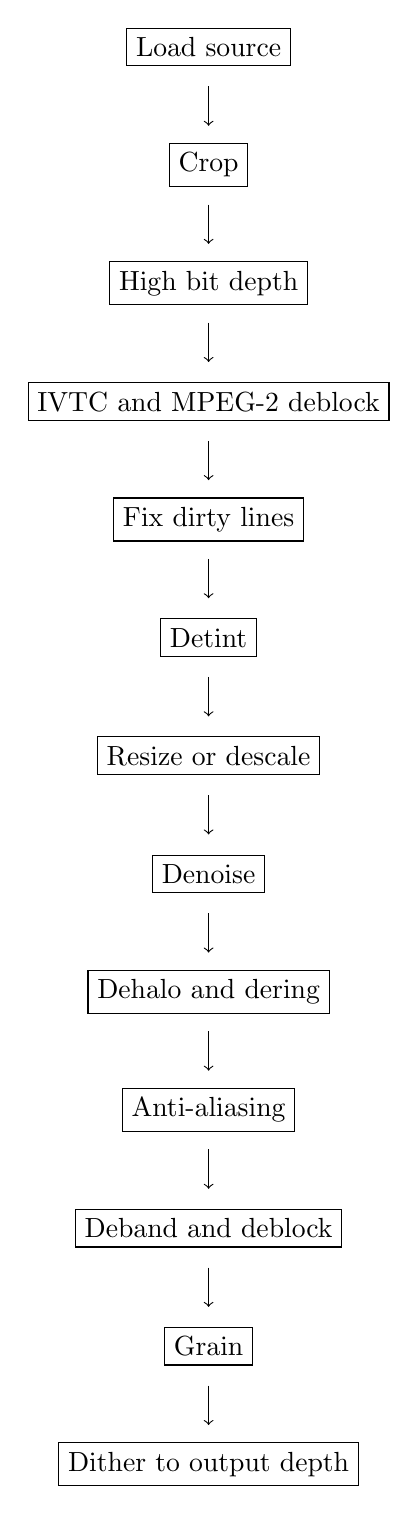
\begin{tikzpicture}
\node[draw] at (0, 0) {Load source};
\draw[->] (0, -0.5) -- (0, -1);
\node[draw] at (0, -1.5) {Crop};
\draw[->] (0, -2) -- (0, -2.5);
\node[draw] at (0, -3) {High bit depth};
\draw[->] (0, -3.5) -- (0, -4);
\node[draw] at (0, -4.5) {IVTC and MPEG-2 deblock};
\draw[->] (0, -5) -- (0, -5.5);
\node[draw] at (0, -6) {Fix dirty lines};
\draw[->] (0, -6.5) -- (0, -7);
\node[draw] at (0, -7.5) {Detint};
\draw[->] (0, -8) -- (0, -8.5);
\node[draw] at (0, -9) {Resize or descale};
\draw[->] (0, -9.5) -- (0, -10);
\node[draw] at (0, -10.5) {Denoise};
\draw[->] (0, -11) -- (0, -11.5);
\node[draw] at (0, -12) {Dehalo and dering};
\draw[->] (0, -12.5) -- (0, -13);
\node[draw] at (0, -13.5) {Anti-aliasing};
\draw[->] (0, -14) -- (0, -14.5);
\node[draw] at (0, -15) {Deband and deblock};
\draw[->] (0, -15.5) -- (0, -16);
\node[draw] at (0, -16.5) {Grain};
\draw[->] (0, -17) -- (0, -17.5);
\node[draw] at (0, -18) {Dither to output depth};
\end{tikzpicture}
\caption{Recommended order in which to apply each filter. Denoising may have to be done before resizing in some cases.}\label{fig:13}
\end{figure}

\pagebreak

\subsubsection{Example Scripts}

Mirai (2018):
\begin{lstlisting}
import vapoursynth as vs
core = vs.get_core()
import fvsfunc as fvf
import mvsfunc as mvf
import kagefunc as kgf
import vsTAAmbk as taa
import havsfunc as haf
from debandmask import *
from rekt import *
from adptvgrnMod import *

src = core.ffms2.Source("")

# Going up to 16-bit, as I like to work in this depth.
b16 = mvf.Depth(src, 16).std.Crop(top=20, bottom=22)

# Filling the first row and filling the chroma of the first two rows.
fb1 = core.fb.FillBorders(b16, top=1)
fb2 = core.fb.FillBorders(b16, top=2)
b16 = core.std.Merge(fb1, fb2, [0,1])

# Super light denoising.  No point in BM3D for denoising this weak.
b16 = core.knlm.KNLMeansCL(b16, a=3, h=0.1, d=2, device_type='gpu', device_id=0, channels='Y')
b16 = core.knlm.KNLMeansCL(b16, a=2, h=0.2, d=1, device_type='gpu', device_id=0, channels='UV')

# Soft dehalo. 
b16 = haf.FineDehalo(b16, rx=2.0, thmi=80, thma=128, thlimi=25, thlima=100, darkstr=0.5, brightstr=0.5)

# Dirty lines during credits.  Cleaning edges, then halos.
cf = core.std.Crop(b16, left=94, top=292, right=1018, bottom=290).fb.FillBorders(top=1, left=1, bottom=1).edgefixer.ContinuityFixer(left=[2, 2, 2], top=[2, 2, 2], right=2, bottom= [0, 2, 2], radius=15)
fb = rekt_fast(b16, lambda x: core.fb.FillBorders(x, left=2, top=2, right=1, bottom=2).std.Merge(cf, [1,0]), left=94, top=292, right=1018, bottom=290)
dh = rekt_fast(fb, lambda x: haf.FineDehalo(x, rx=2.0, thmi=80, thma=128, thlimi=25, thlima=100, darkstr=0.5, brightstr=2.3), left=94, top=292, right=1018, bottom=290)
sf = fvf.rfs(b16, dh, "[1434 2296]")

cf = core.std.Crop(b16, left=94, top=302, right=1018, bottom=300).fb.FillBorders(left=1).edgefixer.ContinuityFixer(left=[2, 2, 2], top=1, right=1, bottom= [1, 2, 2], radius=5)
fb = rekt_fast(b16, lambda x: core.fb.FillBorders(x, left=2, top=1, right=1, bottom=2).std.Merge(cf, [1,0]), left=94, top=302, right=1018, bottom=300)
dh = rekt_fast(fb, lambda x: haf.FineDehalo(x, rx=2.0, thmi=80, thma=128, thlimi=25, thlima=100, darkstr=0.5, brightstr=1.5), left=94, top=302, right=1018, bottom=300)
sf = fvf.rfs(sf, dh, "[133711 135117] [135360 136057] [136143 137216] [137282 138288] [138377 138757] [138820 140782]")

cf = core.std.Crop(b16, left=94, top=302, right=1018, bottom=300).fb.FillBorders(left=1).edgefixer.ContinuityFixer(left=[2, 2, 2], top=1, right=1, bottom= [1, 2, 2], radius=5)
fb = rekt_fast(b16, lambda x: core.fb.FillBorders(x, left=2, top=1, right=1, bottom=2).std.Merge(cf, [1,0]), left=94, top=302, right=1018, bottom=300)
dh = rekt_fast(fb, lambda x: haf.FineDehalo(x, rx=2.0, thmi=80, thma=128, thlimi=25, thlima=100, darkstr=0.5, brightstr=1.5).f3kdb.Deband(y=48, cb=0, cr=0, range=5, grainy=64, grainc=32, output_depth=16, keep_tv_range=True), left=94, top=302, right=1018, bottom=300)
sf = fvf.rfs(sf, dh, "[135118 135296] [138305 138376]")

mask = core.std.ShufflePlanes(b16, 0, vs.GRAY).std.Trim(2400, 2401) * src.num_frames
mask = rekt(mask, core.std.BlankClip(b16, 1920, 1038, format=vs.GRAY16), left=666, top=292, right=1114, bottom=744)
dh_lim = core.std.MaskedMerge(dh, b16, mask)
sf = fvf.rfs(sf, dh_lim, "[2297 2329]")

# 4:3 cropped scene.  Replacing borders with my own black borders in order to keep them from having a different shade of black.
crop = core.std.Crop(b16, left=254, right=254)
fb = core.fb.FillBorders(crop, left=1, right=1).std.Merge(crop, [1,0]).edgefixer.ContinuityFixer(left=1, right=1, top=0, bottom=0, radius=50).std.AddBorders(left=254, right=254, color=[4096, 32768, 32768])
sf = fvf.rfs(sf, fb, "[33448 34196]")

# Placebo edgemask binarized so we only get the obvious edges, then inflated.
mask = kgf.retinex_edgemask(b16).std.Binarize(65500).std.Maximum().std.Inflate()

# Strong aliasing.
aa = taa.TAAmbk(b16, aatype=2, mtype=0, opencl=False)
aa = core.std.MaskedMerge(b16, aa, mask)
sf = fvf.ReplaceFramesSimple(sf, aa, mappings="[4225 4727] [18340 18387] [129780 131148]")

# Mild aliasing.
aa = taa.TAAmbk(b16, aatype=3, mtype=0, opencl=False)
aa = core.std.MaskedMerge(b16, aa, mask)
sf = fvf.ReplaceFramesSimple(sf, aa, mappings="[55394 55451] [55649 55782] [120840 120901]")

# Very strong aliasing.
aa = taa.TAAmbk(b16, aatype=6, mtype=0, repair=16)
aa = core.std.MaskedMerge(b16, aa, mask)
sf = fvf.ReplaceFramesSimple(sf, aa, mappings="[107405 107462]")

# Strong aliasing that I tried to fix with a terrible mask.
mask = kgf.retinex_edgemask(b16).std.Binarize(65500).std.Maximum().std.Minimum(
	coordinates=[1,0,1,0,0,1,0,1]).std.Deflate().std.Deflate()
aa = taa.TAAmbk(b16, aatype=6, mtype=0, opencl=False)
aa = core.std.MaskedMerge(b16, aa, mask)
sf = fvf.ReplaceFramesSimple(sf, aa, mappings="[55510 55580]")

# I simply marked this, it would require a lot of work, so I just decided against doing this.
#sf = fvf.rfs(sf, ?, "[65880 66478]")
#sf = fvf.rfs(sf, ?, "[120902 121051] [121790 121905] [122388 122528] [123038 123153] [126686 126812] [128740 128953]") #Banding? [121063 121095] [121906 121968] [122530 122576]

# Graining an area with no grain.
gr = adptvgrnMod(b16, strength=2.5, size=1.25, sharp=35, static=False, luma_scaling=3, grain_chroma=False)
sf = fvf.rfs(sf, gr, "[120840 120901]")

# Debanding with the standard debandmask.  All of these debanding areas had almost no grain, so I added some on top.
dbmask = debandmask(b16, lo=6144, hi=12288, lothr=320, hithr=384, mrad=2)
deband = core.f3kdb.Deband(b16, y=34, cb=0, cr=0, range=10, grainy=16, grainc=8, output_depth=16, keep_tv_range=True)
merge = core.std.MaskedMerge(deband, b16, dbmask)
merge = adptvgrnMod(merge, strength=2, size=1.5, sharp=25, static=False, luma_scaling=5, grain_chroma=True)
sf = fvf.rfs(sf, merge, "[3174 3254] [3540 3655] [7463 7749] [41056 41597] [63482 64106] [91033 91164]")

# Debanding with retinex.
mask = kgf.retinex_edgemask(b16).std.Maximum().std.Inflate().std.Maximum().std.Inflate()
deband = core.f3kdb.Deband(b16, y=48, cb=48, cr=48, range=15, grainy=16, grainc=16, output_depth=16, keep_tv_range=True)
merge = core.std.MaskedMerge(deband, b16, mask)
merge = adptvgrnMod(merge, strength=2.2, size=1.25, sharp=15, static=False, luma_scaling=5, grain_chroma=True)
sf = fvf.rfs(sf, merge, "[77952 78034] [93358 93443]")

# Debanding with gradfun3 mask.
deband = Fag3kdb(b16, thry=54, thrc=54, radiusy=10, radiusc=6, grainy=32, grainc=16)
sf = fvf.rfs(sf, deband, "[25 263]")

# Dithering back to 8-bit.
final = mvf.Depth(sf, 8, dither=7)

# Replacing black areas with a simple black screen in order to keep slight variations from happening.  Usually not necessary, though.
blank = core.std.BlankClip(src.std.Crop(top=20, bottom=22), 1920, 1038, color=[16, 128, 128])
final = fvf.rfs(final, blank, "[0 24] [1352 1433] [58945 59016] [75563 75633] [78351 78421] [81130 81141] [81261 81272] [93967 94062] [99889 99959] [118093 118147] [140928 140951]")

final.set_output()
\end{lstlisting}
Sword Art Online: The Movie - Ordinal Scale (2017):\\\texttt{Sword.Art.Online.The.Movie.Ordinal.Scale.2017.ITA.1080p.BluRay.AC3.x264.D-Z0N3}
\begin{lstlisting}
import vapoursynth as vs
core = vs.get_core()
import fvsfunc as fvf
import kagefunc as kgf
import havsfunc as hvf
import vsTAAmbk as taa
import fag3kdb
import nnedi3_rpow2 as nnrp

src = core.ffms2.Source("")
resize = src # I called this and was too lazy to change it.

# Rescaling a flashback with grain.
dn = core.knlm.KNLMeansCL(src, d=3, a=1, s=0, h=1.5, device_type="gpu", device_id=1, channels="Y")
diff = core.std.MakeDiff(src, dn, planes=[0])
ds = fvf.Debicubic(dn, 1280, 720)
us = nnrp.nnedi3_rpow2(ds, 2, 1920, 1080, kernel="Spline36")
merged = core.std.MergeDiff(us, diff, planes=[0])
src = fvf.ReplaceFramesSimple(resize, merged, mappings="[3418 3507] [3508 5145] [75916 76205] [76253 76323] [77720 77790]")

# Rescaling a flashback without grain.
ds = fvf.DescaleAA(dn, 1280, 720).std.MergeDiff(diff, planes=[0])
src = fvf.ReplaceFramesSimple(src, ds, mappings="[3298 3417]")

# Going to 16-bit.  The above parts are in 8-bit because I was scared of performance issues.
src = fvf.Depth(src, 16)

# I like to establish a separate variable for 16-bit and leave src for 8-bit, but didn't do that here.  This is so I could copy-paste commands.
b16 = src

# Anti-aliasing.  As you might be able to tell, the crop and stacking could now be replaced by rekt_fast or simply rektaa.
aa = core.std.Crop(b16, left=400, right=1006)
aa = taa.TAAmbk(aa, aatype=-3, preaa=-1, strength=0, mtype=2, opencl=True)
left = core.std.Crop(b16, right=1920 - 400)
right = core.std.Crop(b16, left=1920 - 1006)
aa = core.std.StackHorizontal([left, aa, right]).std.Crop(top=208, bottom=456)
top = core.std.Crop(b16, bottom=1080 - 208)
bottom = core.std.Crop(b16, top=1080 - 456)
aa = core.std.StackVertical([top, aa, bottom])
sfaa = fvf.ReplaceFramesSimple(b16, aa, mappings="[42583 42813] [58812 59050] [65211 65281] [92132 92274]")

# Debanding with a standard ass mask.
db = b16.f3kdb.Deband( range=15, y=60, cb=60, cr=60, grainy=22, grainc=22, output_depth=16)
mask = kgf.retinex_edgemask(b16).std.Inflate() 
merged = core.std.MaskedMerge(db, b16, mask)
sfdb = fvf.ReplaceFramesSimple(sfaa, merged, mappings="[3508 3603] [17600 17706] [41865 42113] [76922 77488] [78444 78598] [81054 81280] [150853 150933] [152057 152288] [152324 152424] [152443 152508] [152521 152686] [171669 172433] [172561 172643] [170283 170557]")

# Debanding values that were outside of the range of 10000-25000.
db = b16.f3kdb.Deband(range=10, y=160, cb=0, cr=0, grainy=28, grainc=0, output_depth=16)
mask = core.std.ShufflePlanes(b16, 0, vs.GRAY).std.Expr("x 10000 < x 25000 > or x 10 * x 10 / ?")
merged = core.std.MaskedMerge(db, b16, mask)
sfdb = fvf.ReplaceFramesSimple(sfdb, merged, mappings=" [96133 96273]")

# Fixing dirty lines during credits.  Again, rekt_fast would've been useful back then.
bot = core.std.Crop(sfdb, top=1080 - 330)
middle = core.std.Crop(sfdb, top=318, bottom=330).edgefixer.ContinuityFixer(top=1, bottom=1, left=0, right=0, radius=5)
fb = core.fb.FillBorders(middle, top=2, bottom=2)
middle = core.std.Merge(fb, middle, [1, 0])
top = core.std.Crop(sfdb, bottom=1080 - 318)
merge = core.std.StackVertical([top, middle, bot])
right = core.std.Crop(merge, left=1920 - 134)
middle = core.std.Crop(merge, left=1018, right=134).edgefixer.ContinuityFixer(left=2, right=2, top=0, bottom=0, radius=5)
fb = core.fb.FillBorders(middle, left=2, right=2)
middle = core.std.Merge(fb, middle, [1, 0])
left = core.std.Crop(merge, right=1920 - 1018)
merge = core.std.StackHorizontal([left, middle, right])
sfc = fvf.ReplaceFramesSimple(sfdb, merge, mappings="[165067 167168] [167403 169466] [169842 170557] [170558 171041]")

# Dithering the result back to 8-bit.
final = fvf.Depth(sfc, 8)

final.set_output()

\end{lstlisting}

BTS - Blood, Sweat and Tears\\
\texttt{BTS - Blood, Sweat \& Tears 2016 1080p ProRes FLAC 2.0 AVC x264 10-bit - A.R.M.Y}\\
A Quick explanation of \texttt{bandmask}\footnote{\url{https://gitlab.com/snippets/1904934}}:\\
Edge masks work by finding areas where gradients are large, so the most simple convolution is
\[
\begin{bmatrix}
0 & 0 & 0 \\
1 & 0 & -1 \\
0 & 0 & 0 
\end{bmatrix},
\]
meaning we're checking the difference between the pixel to the left and the pixel to the right.
We can move the subtraction to identify areas with no grain by checking the difference with the original pixel:
\[
\begin{bmatrix}
0 & 0 & 0 \\
1 & -1 & 0 \\
0 & 0 & 0
\end{bmatrix}
\]
This isn't exactly what's happening here, though; we're performing the subtraction after multiple iterations of the convolution, so we get the gradient over a larger number of pixels.  We then binarize this, minimize to remove noise, then maximize again.
\begin{lstlisting}
import vapoursynth as vs
core = vs.get_core()
import fvsfunc as fvf
import kagefunc as kgf
import havsfunc as hvf
from adptvgrnMod import *
from rekt import *
from bandmask import *

# Load, go to high bit depth, and crop.
src = core.ffms2.Source("Blood, Sweat & Tears 피땀눈물_BTS 방탄소년단-187617728.mov")
hbd = fvf.Depth(src, 16)
crp = hbd.std.Crop(top=134, bottom=134)

# One scene has four lines missing at the bottom and dirty lines elsewhere.
# Every plane was fixed individually.
acr = crp.std.Crop(bottom=4)
ycr = acr.std.ShufflePlanes(0, vs.GRAY)
ucr = acr.std.ShufflePlanes(1, vs.GRAY)
vcr = acr.std.ShufflePlanes(2, vs.GRAY)

ufx = rektlvls(ucr, [ucr.height - 2], [-6.5], prot_val=0).fb.FillBorders(top=1, mode="fillmargins").cf.ContinuityFixer(bottom=1, radius=3)
vfx = vcr.cf.ContinuityFixer(bottom=3, radius=5).fb.FillBorders(bottom=2, top=1, mode="fillmargins")
lvl = rektlvls(ycr, [ycr.height - 2, ycr.height - 3], [-30, -6], prot_val=10)
fmg = lvl.cf.ContinuityFixer(bottom=2, radius=3).fb.FillBorders(bottom=1, top=1, mode="fillmargins")

# Merge fixes and change subsampling to 4:2:0, then add borders.
acr = core.std.ShufflePlanes([fmg, ufx, vfx], [0, 0, 0], vs.YUV)
rsz = acr.resize.Spline36(format=vs.YUV420P16)
adb = rsz.std.AddBorders(bottom=4)

# Rest of the video only has one line missing top and bottom.  Fixed and subsampling changed.
fmg = crp.fb.FillBorders(top=1, bottom=1, mode="fillmargins")
rsz = fmg.resize.Spline36(format=vs.YUV420P16)

# Spliced the fix in with the rest.
trm = rsz.std.Trim(0, 5232) + adb.std.Trim(5233, 5260) + rsz.std.Trim(5261)

# Luma debanding during a couple scenes with graining.
dbn = trm.f3kdb.Deband(y=64, cr=0, cb=0, range=6, grainy=0, grainc=0, output_depth=16)
msk = kgf.retinex_edgemask(trm).std.Binarize(11000).std.Maximum().std.Inflate()
mrg = dbn.std.MaskedMerge(trm, msk)
grn = adptvgrnMod(mrg, size=1.4, sharp=90, luma_scaling=4, grainer=lambda x: core.grain.Add(x, var=1.6, uvar=1.0, constant=False))
snf = fvf.rfs(trm, grn, "[1612 1616] [7779 7794]")

# Some blocking was fixed with bandmask, since no edges were present.
bmk = bandmask(trm, 200).std.Crop(top=500).std.AddBorders(top=500)
grn = adptvgrnMod(dbn, size=1.3, sharp=90, luma_scaling=4, grainer=lambda x: core.grain.Add(x, var=.4, uvar=.3, constant=False))
mrg = trm.std.MaskedMerge(grn, bmk)
snf = fvf.rfs(snf, mrg, "[7964 7980] [8009 8018]")

# One scene has missing grain, so used bandmask and adptvgrnMod to fix this.
# I got frustrated and started copy pasting random Maximize/Inflate calls.
bmk = bandmask(trm, thr=300)
lmk = trm.std.ShufflePlanes(0, vs.GRAY).std.Binarize(55000).std.Maximum().std.Maximum().std.Maximum().std.Maximum().std.Maximum()
gmk = core.std.Expr([bmk, lmk], "x y -").std.Crop(bottom=225, top=100).std.AddBorders(bottom=225, top=100).std.Maximum().std.Inflate().std.Maximum().std.Inflate().std.Maximum().std.Maximum().std.Maximum().std.Maximum().std.Maximum().std.Maximum().std.Inflate().std.Inflate().std.Inflate().std.Inflate().std.Inflate().std.Inflate().std.Inflate()
gmk = kgf.iterate(gmk, core.std.Maximum, 3)
grn = adptvgrnMod(trm, size=1.2, sharp=80, luma_scaling=1, grainer=lambda x: core.grain.Add(x, var=1.4, uvar=1.0, constant=False))
mrg = core.std.MaskedMerge(trm, grn, gmk)
snf = fvf.rfs(snf, mrg, "[7579 7778]")

# Dehalo on one scene.
fdh = hvf.FineDehalo(trm)
grn = adptvgrnMod(fdh, size=1.2, sharp=80, luma_scaling=8, grainer=lambda x: core.grain.Add(x, var=.8, uvar=.5, constant=False))
snf = fvf.rfs(snf, grn, "[6523 6591]")

# Dither to output depth.
out = fvf.Depth(snf, 10)

out.set_output()
\end{lstlisting}

Other fun scripts to read through:
\begin{itemize}
\item \url{https://gist.github.com/blaze077/9025d2c1a9a59d63f0168e5fd6f9cd31} Kaiji episode 1 by blaze077
\item \url{https://pastebin.com/q469qUcU} How to IVTC by eXmendiC
\item \url{https://github.com/Beatrice-Raws/encode-scripts} Various scripts by Beatrice-Raws
\item \url{https://github.com/LightArrowsEXE/Encoding-Projects} Various scripts by LightArrowsEXE
\item \url{https://git.kageru.moe/kageru/vs-scripts/src/branch/master/abyss1.py} Made in Abyss episode 1 by kageru
\item \url{https://pastebin.com/JB8aEGgf} Something by Nginx from TnP
\item \url{https://github.com/Ichunjo/encode-scripts} - Various scripts by Vard$\ddot{\textrm{e}}$
\item \url{https://git.concertos.live/OpusGang/EncodeScripts} - Various crowdsourced scripts
\item Please send me more of these.  It's super hard to find decent scripts, especially live action stuff.
\end{itemize}

\subsubsection{Forum and Blog Posts}\label{posts}
Public:
\begin{itemize}
\item Descaling: \url{https://guide.encode.moe/encoding/descaling.html}
\item Masking: \url{https://guide.encode.moe/encoding/masking-limiting-etc.html}
\item Adaptive grain: \url{https://blog.kageru.moe/legacy/adaptivegrain.html}
\item Kirsch and retinex edge masks: \url{https://blog.kageru.moe/legacy/edgemasks.html}
\item Denoisers: \url{https://blog.kageru.moe/legacy/grain.html}
\end{itemize}
Private:
\begin{itemize}
\item Explanation of bandmask: \url{https://i.fiery.me/Atwjs.png}
\item Explanation of adptvgrnMod's graining params: \url{https://i.fiery.me/bELRN.png}
\item Automating debanding (without \texttt{banddtct}): \url{https://awesome-hd.me/forums.php?action=viewthread&threadid=27426&post=4#post201503}\footnote{\url{https://privatebin.at/?c7bb6074f0b40a6f\#98AThVWCCTjzVwGieifezXweCZ2EEKzKx2MU3gZJ87mu}}
\item Spotting double range compression: \url{https://passthepopcorn.me/forums.php?action=viewthread&threadid=9197&postid=1622921#post1622921}\footnote{\url{https://privatebin.at/?5f86bab33960876c\#FXTAkApNbzQabAugep4jDYzp6nK4qYDthJaZgG2acVrQ}}
\item A take on when to use which method to fix dirty lines (Fixer is ContinuityFixer): \url{https://passthepopcorn.me/forums.php?action=viewthread&threadid=35149&postid=1656050#post1656050}\footnote{\url{https://privatebin.at/?aebe974a92324a02\#4QCrc8jhbSNojzr5gYZVsjG3rwPX8DVjdNk3T6eENySw}}
\item Using \texttt{banddtct} and \texttt{dirtdtct}: \url{https://git.concertos.live/AHD/awsmfunc/issues/13#issuecomment-62}
\end{itemize}

\subsection{x264 and x265}

The two main video encoders we recommend are x264 and x265.  While x265 should technically be superior, as it's the newer encoder, they both do have their upsides and downsides.

Being the more mature codec, x264 is more consistent, meaning you're less likely to be left with random scenes inexplicably looking awful.  It also has better hardware support and is far faster to encode.  The difference in encode speeds is usually at least a factor of 5.

On the flipside, x265 has the advantage that it is capable of storing HDR information and is substantially more efficient, especially simple stuff like anime at low bitrates.

\subsubsection{8-bit and 10-bit Explained}

The two bit depths we recommend considering for x264 are 8-bit and 10-bit.  If you're using x265, just always use 10-bit, as it's better in every way.  With x264, 8-bit has far more hardware compatibility (10-bit has practically none) and is significantly faster.  However, 10-bit x264 is usually capable of saving quite a bit of space while remaining faster than x265.  Additionally, 10-bit encoding is far better at preserving gradients (i.\@e.\ you won't have to be as afraid of banding reoccurring), which makes it very popular for encoding grain-free content such as anime.

\subsubsection{x264 Settings}

From the AHD guide (hardware compatibility stuff is in gray, a few items changed):\\
\textbf{General settings:}
\begin{itemize}
\item \textcolor{gray}{\texttt{-{}-level 4.1} for DXVA.}
\item \texttt{-{}-b-adapt 2} uses the best algorithm (that x264 has) to decide how B frames are placed.
\item \texttt{-{}-min-keyint} should typically be the frame rate of your video, e.g. if you were encoding 23.976\,fps content, then you use 24. This is setting the minimum distance between I-frames.
\item \textcolor{gray}{\texttt{-{}-vbv-bufsize 78125 -{}-vbv-maxrate 62500} for DXVA (The old guide used lower values to account for the possibility of writing the encode to BD for playback, this is no longer a consideration as other settings break this compatibility. The new values are the max level 4.1 can do, if your device breaks because of this the encode is not at fault, your device doesn't meet DXVA spec).}
\item \texttt{-{}-rc-lookahead 250} if using mbtree, 60 or higher else. This sets how many frames ahead x264 can look, which is critical for mbtree. You need lots of memory for this. (Personally I just leave this at 250 now as the impact on memory usage is 2\,GB or so.)  Definitely lower this if you're encoding without mbtree and have a lot of ReplaceFramesSimple calls in your script.
\item \texttt{-{}-me umh} is the lowest you should go.  If your CPU is fast enough, you might endure the slowdown from tesa. esa takes as much time as tesa without any benefit, so if you want to slow down your encode to try and catch more movement vectors, just use tesa, although the increase is not necessarily always worth it. This isn't really a setting you need to test, but on tough sources, you might squeeze some more performance out of x264 if you use tesa.
\item \texttt{-{}-direct auto} will automatically choose the prediction mode (spatial/temporal)
\item \texttt{-{}-subme 10} or \texttt{11} (personally I just set this to 11 the difference in encode speed is within 3-4\%)
\item \texttt{-{}-trellis 2}
\item \texttt{-{}-no-dct-decimate} dct-decimate is a speed up that sacrifices quality.  Just leave it off, since your computers can likely handle it.
\item \texttt{-{}-no-fast-pskip} Similar to the above.
\item \texttt{-{}-preset veryslow} or \texttt{placebo}, although the stuff we're changing will make veryslow be placebo, anyway.
\end{itemize}
\textbf{Source-specific settings:}
\begin{itemize}
\item \texttt{-{}-bitrate} / \texttt{-{}-crf} Bitrate is in Kbps (Kilobits per second) and CRF takes a float, where lower is better quality. This is the most important setting you have; bitstarve an encode and it is guaranteed to look like crap. Use too many bits and you've got bloat (and if people wanted to download massive files, they would get a remux). Of course, the bitrate need can vary drastically depending on the source.
\item \texttt{-{}-deblock -3:-3} to \texttt{1:1}. For live action, most people just stick with -3:-3.  For anime, values between -3:-2 and 0:0 are common, with offsets of 1 between the two values being the norm (common values are -1:0, 0:-1, and -2:-1).
\item \texttt{-{}-qcomp 0.6} (default) to \texttt{0.8} might prove useful. Don't set this too high or too low, or the overall quality of your encode will suffer. This setting has a heavy effect on mbtree. A higher qcomp value will make mbtree weaker, hence something around 0.80 is usually optimal for anime. \texttt{-{}-qcomp 0} will cause a constant bitrate, while \texttt{-{}-qcomp 1} will cause a constant quantizer.
\item \texttt{-{}-aq-mode 1} to \texttt{3}: 1 distributes bits on a per frame basis, 2 tends to allocate more bits to the foreground and can distribute bits in a small range of frames, 3 is a modified version of 2 that attempts to allocate more bits to dark parts of the frames. The only way to know what's best for sure it to test.  Almost every source ends up looking best with aq-mode 3, however.
\item \texttt{-{}-aq-strength 0.5} to \texttt{1.3} are worth trying. Higher values might help with blocking. Lower values will tend to allocate more bits to the foreground, similar to aq-mode 2. This setting drastically affects the bitrate when encoding with CRF, so it might be worthwhile to test this setting with 2 pass if you intend on using CRF for the final encode.
\item \texttt{-{}-merange 24} (the lowest that should ever be used) to \texttt{64}, setting this too high can hurt (more than 128), 32 or 48 will be fine for most encodes. In general, 32-48 for 1080p and 32 for 720p (when using umh) for movies with lots of motion this can help (e.g. action movies). Talking heads can get away with low values like 24. The impact on encode speed is noticeable but not horrible. I prefer to use 48 for 1080p and 32 for 720p when using umh or 32 for 1080p and 32 for 720p when using tesa.
\item \texttt{-{}-no-mbtree} I highly recommend testing with both mbtree enabled and disabled, as generally it will result in two very different encodes. mbtree basically attempts to degrade the quality of blocks rather than frames, so that only the unimportant parts of a frame get less bits. To do this, it needs to know how often a block is referenced later, which is why \texttt{-{}-rc-lookahead} should be set to 250. Useful for things with static backgrounds, like anime. Or for things where you've used a high qcomp (.75 or above) and mbtree will have a lowered impact.  When testing whether this is a decent option, you'll likely have to retest every setting, especially qcomp, psy-rd, and ipratio.
\item \texttt{-{}-ipratio 1.15} to \texttt{1.40}, with 1.30 usually being the go-to option.  This is the bitrate allocation ratio between I and P frames.
\item \texttt{-{}-pbratio 1.05} to \texttt{1.30}, with 1.20 being the usual go-to.  This is the bitrate allocation ratio between P and B frames.  This value should always be around 0.10 lower than -{}-ipratio, so lower it while testing ipratio.  If you're using mbtree, this setting will have no affect, as mbtree determines it itself.
\item \texttt{-{}-psy-rd 0.40:0 to 1.15:0}: 0.95:0 to 1.15:0 for live action. The first number is psy-rd strength, second is psy-trellis strength. This tries to keep x264 from making things blurry and instead keep the complexity. For anime, between 0.40 and 1.00:0.00 is the usual range.  Psy-trellis usually introduces a lot of ringing, but can help with maintaining dither.  You can try values between 0.00 and 0.15 for live action and try values up to 0.50 for anime, although you'll usually get better results if you raise your aq-strength instead.
\item \texttt{-{}-bframes 6} to \texttt{16}, This is setting the maximum amount of consecutive P frames that can be replaced with B frames. Test with 16 for your first test run, and set according to the x264 log:

\texttt{x264 [info]: consecutive B-frames:  1.0\%  0.0\%  0.0\%  0.0\% 14.9\% 23.8\% 13.9\% 15.8\%  8.9\%  9.9\%  0.0\% 11.9\%  0.0\%  0.0\%  0.0\%  0.0\%  0.0\%}

Start counting with the first percentage as 0 and choose the highest number with more than 1\%, which is 11 in this example. (Or just leave this at 16 as allowing more bframes will not harm your encode and will aid in compression, the impact on speed isn't that enormous.)
\item -{}-ref set the number of previous frames each P frame can use as references.  If you don't care about hardware compatibility (and/or are doing a 10-bit encode), set this to 16.  The impact on performance is quite large, but it's worth it most of the time.  \textcolor{gray}{Calculate the number you can use or if you're using the provided CLI inputs at the end of this it will be calculated for you by x264. Always use the max that you can.\\
The max \texttt{-{}-ref} value can be calculated as follows:\\
For \texttt{-{}-level 4.1}, according to the H.264 standard, the max DPB (Decoded Picture Buffer) size is 12,288 kilobytes.\\
Since each frame is stored in YV12 format, or 1.5 bytes per pixel, a 1920x1088 frame is $1920 \times 1088 \times 1.5 = 3133440\,\mathrm{bytes} = 3060$\,kilobytes.\\
$12,288 \div 3060\,\mathrm{kilobytes} = 4.01568627$, so you can use a maximum of 4 reference frames.\\
Remember, round both dimensions up to a mod16 value when doing the math, even if you're not encoding mod16!\\
Let's do the math for 1920x800.\\
$1920 \times 800 \times 1.5 = 2304000\,\mathrm{bytes} = 2250$\,kilobytes. $12,288 \div 2250\,\mathrm{kilobytes} = 5.45777778$, so you can use a maximum of 5 reference frames Note that these conversions use base 2, so 1\,Kilobyte == 1024\,bytes. If you get the math wrong, that's okay too - x264 will display a warning if you use too many, so you'll know if you need to change it.}

\item \texttt{-{}-zones} is quite useful for debanding and blocking, as these areas require a larger bitrate to maintain transparency.  The syntax is \\\texttt{-{}-zones 0,100,crf=10/101,200,crf=15} or\\ \texttt{-{}-zones 0,100,b=5/101,200,b=10} with \texttt{b} being a bitrate multiplier in this case.  You can also use this for areas that don't get enough bits allocated.  Especially common areas are darker scenes or scenes with lots of reds.  Fades can also suffer from bitstarving and require zoning.  One can also lower the bitrate during credits to save that little something.
\item \texttt{-{}-output-depth 8} or \texttt{10} depending on what you're encoding in.
\item \texttt{-{}-output-csp i444} if you're encoding 4:4:4, else leave this out.
\end{itemize}

\subsubsection{x265 Settings}

The documentation here is very good, so I'll just go over recommended values:\\
\textbf{Source-independent settings:}
\begin{itemize}
\item \texttt{-{}-preset veryslow} or \texttt{slower}
\item \texttt{-{}-no-rect} for slower computers.  There's a slight chance it'll prove useful, but it probably isn't worth it.
\item \texttt{-{}-no-amp} is similar to \texttt{rect}, although it seems to be slightly more useful.
\item \texttt{-{}-no-open-gop}
\item \texttt{-{}-no-cutree} since this seems to be a poor implementation of \texttt{mbtree}.
\item \texttt{-{}-no-rskip} \texttt{rskip} is a speed up that gives up some quality, so it's worth considering with bad CPUs.
\item \texttt{-{}-no-sao} because \texttt{sao} is one of the stupidest things in x265.
\item \texttt{-{}-ctu 64}
\item \texttt{-{}-min-cu-size 8}
\item \texttt{-{}-rdoq-level 2}
\item \texttt{-{}-max-merge 5}
\item \texttt{-{}-rc-lookahead 60} although it's irrelevant as long as it's larger than min-keyint
\item \texttt{-{}-ref 6} for good CPUs, something like \texttt{4} for worse ones.
\item \texttt{-{}-bframes 16} or whatever your final bframes log output says.
\item \texttt{-{}-rd 3} or \texttt{4} (they're currently the same)
\item \texttt{-{}-subme 5}.  You can also change this to \texttt{7}, but this is known to sharpen.
\item \texttt{-{}-merange 57} just don't go below \texttt{32} and you should be fine.
\item \texttt{-{}-high-tier}
\item \texttt{-{}-range limited}
\item \texttt{-{}-aud}
\item \texttt{-{}-repeat-headers}
\end{itemize}
\textbf{Source-dependent settings:}
\begin{itemize}
\item \texttt{-{}-colorprim 9} for HDR, \texttt{1} for SDR.
\item \texttt{-{}-colormatrix 9} for HDR, \texttt{1} for SDR.
\item \texttt{-{}-transfer 16} for HDR, \texttt{1} for SDR.
\item \texttt{-{}-hdr10} for HDR.
\item \texttt{-{}-hdr10-opt} for 4:2:0 HDR, \texttt{-{}-no-hdr10-opt} for 4:4:4 HDR and SDR.
\item \texttt{-{}-master-display\\ "G(8500,39850)B(6550,2300)R(35400,14600)WP(15635,16450)L(10000000,20)"} with the values for L coming from your source's MediaInfo output.
\item \texttt{-{}-max-cll "711,617"} again from your source's MediaInfo.
\item \texttt{-{}-cbqpoffs} and \texttt{-{}-crqpoffs} should usually be between -3 and 0.  This sets an offset between the bitrate applied to the luma and the chroma planes.
\item \texttt{-{}-qcomp} between \texttt{0.60} and \texttt{0.80}.
\item \texttt{-{}-aq-mode 4}, \texttt{3}, \texttt{2}, \texttt{1}, or \texttt{-{}-hevc-aq} with \texttt{4} and \texttt{3} usually being the two best options.
\item \texttt{-{}-aq-strength} between \texttt{0.80} and \texttt{1.50}.
\item \texttt{-{}-deblock -4:-4} to \texttt{0:0}, as with x264.  You can default \texttt{-3:-3} with live action.
\item \texttt{-{}-ipratio} and \texttt{-{}-pbratio} same as x264 again.
\item \texttt{-{}-psy-rd 0.50} to \texttt{2.00}, similar-ish to x264.
\item \texttt{-{}-psy-rdoq} anything from \texttt{0.00} to \texttt{2.00} usually.
\item \texttt{-{}-no-strong-intra-smoothing} on sharp/grainy content, you can leave this on for blurry content, as it's an additional blur that'll help prevent banding.
\item \texttt{-{}-output-depth 10} for 10-bit output.
\end{itemize}
\textbf{Experimental settings:}
\begin{itemize}
\item \texttt{-{}-scenecut-aware-qp}
\item \texttt{-{}-scenecut-window 550}
\item \texttt{-{}-max-qp-delta 2}
\item \texttt{-{}-hist-scenecut}
\item \texttt{-{}-hist-threshold 0.02}
\end{itemize}

\subsection{Testing Settings}

To start off, you'll want to select a smaller region of your video file to use as reference, since testing on the entire thing would take forever.  The recommended way of doing this is by using \texttt{awsmfunc}'s \texttt{SelectRangeEvery}:
\begin{lstlisting}
import awsmfunc as awf
out = awf.SelectRangeEvery(clip, every=15000, length=250, offset=[1000, 5000])
\end{lstlisting}
Here, the first number is the offset between sections, the second one is the length of each section, and the offset array is the offset from start and end.

You'll want to use a decently long clip (a couple thousand frames usually) that includes both dark, bright, static, and action scenes, however, these should be roughly as equally distributed as they are in the entire video.

When testing settings, you should always use 2-pass encoding, as many settings will substantially change the bitrate CRF gets you.  For the final encode, both are fine, although CRF is faster.

To find out what setting is best, compare them all to each other and the source.  You can do so by interleaving them either individually or by a folder via \texttt{awsmfunc}.  You'll usually also want to label them, so you actually know which clip you're looking at:
\begin{lstlisting}
# Load the files before this
src = awf.FrameInfo(src, "Source")
test1 = awf.FrameInfo(test1, "Test 1")
test2 = awf.FrameInfo(test2, "Test 2")
out = core.std.Interleave([src, test1, test2])

# You can also place them all in the same folder and do
src = awf.FrameInfo(src, "Source")
folder = "/path/to/settings_folder"
out = awf.InterleaveDir(src, folder, PrintInfo=True, first=extract, repeat=True
\end{lstlisting}

If you're using \texttt{yuuno}, you can use the following iPython magic to get the preview to switch between two source by hovering over the preview screen:
\begin{lstlisting}
%vspreview --diff
clip_A = core.ffms2.Source("settings/crf/17.0")
clip_A.set_output()
clip_B = core.ffms2.Source("settings/crf/17.5")
clip_B.set_output(1)
\end{lstlisting}

Usually, you'll want to test for the bitrate first.  Just encode at a couple different CRFs and compare them to the source to find the highest CRF value that is indistinguishable from the source.  Now, round the value, preferably down, and switch to 2-pass.  For standard testing, test qcomp (intervals of 0.05), aq-modes, aq-strength (intervals of 0.05), merange (32, 48, and 64), psy-rd (intervals of 0.05), ipratio/pbratio (intervals of 0.05 with distance of 0.10 maintained), and then deblock (intervals of 1).  If you think mbtree could help (i.\@e.\ you're encoding animation), redo this process with mbtree turned on.  You probably won't want to change the order much, but it's certainly possible to do so.

For x265, the order should be qcomp, aq-mode, aq-strength, psy-rd, psy-rdoq, ipratio and pbratio, and then deblock.

If you want that little extra efficiency, you can redo the tests again with smaller intervals surrounding the areas around which value you ended up deciding on for each setting.  It's recommended to do this after you've already done one test of each setting, as they do all have a slight effect on each other.

Once you're done testing the settings with 2-pass, switch back to CRF and repeat the process of finding the highest transparent CRF value.

\section{Audio}

\subsection{SoX}

If your source audio is hi-res (24-bit or >48\,kHz), you may want to consider changing this in order to save space, as hi-res audio is very much placebo for consumers if proper conversion is done.  In order to do this, we recommend \texttt{SoX}.  If you want to convert to 16-bit 48\,kHz, you can use the following input:
\[
\texttt{\$ sox foo.wav -G -b 16 bar.wav -v -L 48000 dither -s -f gesemann}
\]
Use this if your source audio's sample rate is a multiple of 48\,kHz (e.\@g.\ 96\,kHz).  For multiples of 44.1\,kHz, you can simple switch out the number 48000 with 44100.

We recommend doing these conversions for encodes, as higher sample rates are usually more destructive than anything else, and the difference between 24-bit and properly done 16-bit is so small that it'd only be noticeable at extremely high volumes.

\subsection{Lossy Codecs}

\subsubsection{Opus}

Opus, while the most efficient codec and the preferred lossy codec on Concertos, has almost no hardware compatibility.  This is not an issue for anyone using an HTPC, a desktop, a laptop, or even a phone, but users trying to use their Blu-ray players for playback won't be able to play it back.  As we don't care as much about hardware compatibility, this is likely the easiest way to go.  Apart from being the most efficient codec, it's also fully open source, just like FLAC, and works perfectly on every operating system.

The biggest issue with Opus is that it doesn't work with matroska's ordered chapters; however, unless you're encoding something with a lot of the same intros/outros repeated, this shouldn't matter.

In order to encode opus, you need to have \texttt{opus-tools} installed, from there on it's simply
\[
\texttt{\$ opusenc foo.wav bar.opus}
\]
Additionally, you can specify the \texttt{--bitrate} if you don't want to use the (admittedly low) defaults, although Opus automatically detects what should be the optimal target bitrate for it.

\subsubsection{qAAC and fdkaac}

As a close second to Opus in terms of efficiency, qAAC is also a viable option.  Unlike Opus, AAC has a lot more hardware compatibility, especially in stereo.  It also has no issues with ordered chapters.  However, qAAC requires iTunes and, under Unix, wine.  In order to encode the highest quality qAAC, your input would be:
\[
\texttt{qaac.\@exe -V 127 foo.wav bar.m4a}
\]

The \texttt{-V} value specifies quality, with higher numbers being better at \texttt{127} being the maximum.

\subsubsection{Dolby Digital aka. Audio Codec 3}

The king of hardware compatibility is AC-3.  As it was the go-to codec for DVDs, it has very good support on most playback devices.  However, its efficiency is worse than MP3.  If you want to encode this at hoome for hardware compatibility (e.\@g.\ you want to encode something for AHD/HDB/etc), the recommended way of doing this is via Sound Forge (Windows) or Dolby Media Producer (OS X).

In order to encode AC-3 with Sound Forge, open the file (in w64 format), wait for it to index, then go to the Save As option.  From here, select Dolby Digital AC-3 Pro.  Then, select the following options (copied from AHD's guide):
\begin{itemize}
\item Bitstream mode: Main audio service: Complete main
\item Audio coding mode: 3/2 (L, C, R, Ls, Rs) with LFE enabled
\item Sample rate: 48\,kHz
\item Data rate: 640\,kbps
\item Dialog normalization: -32\,dB
\item Do not select Save data in Intel byte order
\item Center mix level: -3\,dB
\item Surround mix level: -3\,dB
\item Do not set copyright bit
\item do not mark as original bitstream
\item Do not include audio production information
\item Do not enable extended bitstream information
\item Do not enable digital de-emphasis
\item Enable DC high-pass filter
\item Enable Bandwidth low-pass filter
\item Enable LFE low-pass filter
\item Do not enable 90-degree phase shift
\item Do not enable 3\,dB attenuation
\item Line mode profile: None
\item RF mode profile: None
\item Do not enable RF overmodulation protection
\end{itemize}

The new E-AC-3 codec has already risen in popularity lately.  What this brings to the table is support for Atmos and more channels.  However, the only crack for the encoder doesn't include Atmos support, and its efficiency is the same as AC-3, as it's simply another layer packed on top.  Because of these reasons, we feel no need to elaborate on how to encode this beyond stating that it requires Dolby Media Producer.

\subsubsection{DTS}

This codec is very common for 1080p private tracker encodes.  Frankly put, it's only because of the bloated bitrate.  DTS actually manages to be worse at 1509\,kbps than AC-3 at 448\,kbps.  Just don't use this.  The only reason to even consider it is laziness, since almost every movie source will feature a DTS core.

\subsection{Lossless Codecs}

\subsubsection{FLAC}

It's free, it's open source, it works everywhere, it's the most efficient.  If you're in stereo or mono, it should be fine in terms of hardware compatibility.  Otherwise, it may have issues with some receivers.
\[
\texttt{\$ flac -{}-compression-level-8 foo.wav bar.flac}
\]

\subsubsection{TrueHD}

%%%%%%%%%%%%
% needhelp %
%%%%%%%%%%%%

This codec is less popular than DTS-HD MA due to inferior hardware support, but it's a bit more efficient, especially at lower bitrates, where the DTS core bloat doesn't inflate the bitrate.  Sadly, due to its inferior hardware compatibility, lots of groups insist on including a separate AC-3 compatibility track.  At Concertos, we'd prefer if you not do this, but understand that this may be necessary to upload elsewhere or simply something you want for hardware compatibility.

I don't know how to encode this.  Ask Scrooge.

\subsubsection{DTS-HD MA}

Because of better support for using the core as fallback, this codec is quite popular for surround sound remuxes.  You can encode it by extracting your track to multiple wavs, one for each channel, then dragging them into the encode suite and clicking the big red encode button.  At Concertos, we don't care for this codec and prefer the use of TrueHD or FLAC.

\section{Muxing}

\subsection{Appending Files}

Sometimes, your encode will crash or you'll want to edit a small portion of an encode.  In situations like these, we can simply append files in \texttt{mkvtoolnix}.  If you just want to add something after another file, just right click the file in the source file field in \texttt{mkvtoolnix}.  

For edits within videos, first locate the appropriate I-frame at the end so you actually encode enough, then encode your segment, open each file in \texttt{mkvtoolnix}, go to the splitting option in the output tab, then set the frames for the part of the video.  Keep in mind counting starts at 1 here unlike Python where it starts at 0.  Do this for the part leading up to and after where you want to add your change, then append them like before.  You can also do this to create a hybrid video remux.

Make sure to check you have all the necessary frames after muxing, as you can easily end up with wrong I-frames being used or an incorrect frame count due to bad trimming if you don't pay perfect attention.

\subsection{Seamless Linking}

Just read this forum post: \url{https://forums.animesuki.com/showthread.php?t=66444}.  There's nothing more that really has to be added.

\section{Recommended Guides and Resources}
\begin{itemize}
	\item Irrational Encoding Wizardry's fansubbing guide: \url{https://guide.encode.moe}
	\item Kageru's blog: \url{https://kageru.moe/blog/}
	\item eXmendiC's filtering guide: \url{https://iamscum.wordpress.com/_test1/_test2/}
	\item AHD Guides
\end{itemize}

\pagebreak

\section{Contributors in Alphabetical Order}

\begin{itemize}
\item Aicha @ D-Z0N3, NSDAB, REEEEEEEE
\item Anon @ Concertos, NSDAB
\item Q2KTyrant @ Concertos
\item Ryuu @ Concertos, NSDAB
\item Scrooge @ Concertos, COC, Fidelity$^\textrm{\tiny{TM}}$
\item xCreamEnte @ EPSiLON, HDBEE, SiGMA
\end{itemize}

%\pagebreak
\begin{figure}[h]
\section{Appendix}
\centering
\includegraphics{Pictures/resizers_down.png}
\caption{Comparison of resizers for downscaling.  The source was downscaled from 1080p to 720p, then cropped.  The parameters were all left at their defaults.}\label{fig:14}
\end{figure}

\begin{figure}[h]
\centering
\includegraphics{Pictures/resizers_up.png}
\caption{Comparison of resizers for upscaling.  The source (Commie encode of Your Name (2016)) was cropped, then upscaled by a factor of 2.}\label{fig:15}
\end{figure}

\begin{figure}[h]
\centering
\includegraphics{Pictures/bicubic_params.png}
\caption{Comparison of bicubic upscales with different parameters.  Keep in mind that these are just small crops of a video, and bicubic upscales will always lead to artifacts, especially aliasing.  Sharp bicubic (b=0, c=1) is especially prone to aliasing artifacts.}\label{fig:22}
\end{figure}

\begin{figure}[h]
\centering
\includegraphics{Pictures/resize_downup.png}
\caption{Comparison of resizers by downscaling and upscaling back to original resolution.  Everything was downscaled to half the source resolution, then upscaled back with \texttt{nnedi3\_rpow2}.  The parameters were all left at their defaults.}\label{fig:20}
\end{figure}

\begin{figure}[h]
\centering
\includegraphics{Pictures/resize_downup2.png}
\caption{Comparison of resizers by downscaling and upscaling back to original resolution.  Everything was downscaled to half the source resolution, then upscaled back with the same resizer.  The parameters were all left at their defaults.}\label{fig:21}
\end{figure}

\begin{figure}[h]
\centering
\includegraphics{Pictures/dither_comparison_8.png}
\caption{Comparison of dither types.  Input source was 8-bit video, dithered up and debanded by \texttt{f3kdb} with 16-bit output, then dithered to 8-bit.}\label{fig:12}
\end{figure}

\begin{figure}[h]
\centering
\includegraphics{Pictures/improper_improper_borders.png}
\caption{Example of why an improper fix of diagonal borders is a bad idea.  Top is source, bottom is Geek's filtered.  Taken from the Geek encode of Hotel Transylvania 2.}\label{fig:26}
\end{figure}

\begin{figure}[h]
\centering
\includegraphics{Pictures/hbd_example.png}
\caption{Comparison of gamma bug fix in 16-bit (right) and 8-bit (left).}\label{fig:flvls}
\end{figure}

\begin{figure}[h]
\begin{minipage}{.5\textwidth}
\centering
\includegraphics[scale=0.5]{Pictures/edgemasks_src.png}
\end{minipage}
\begin{minipage}{.5\textwidth}
\centering
\includegraphics[scale=0.5]{Pictures/edgemasks_prewitt.png}
\end{minipage}
\begin{minipage}{.5\textwidth}
\centering
\includegraphics[scale=0.5]{Pictures/edgemasks_sobel.png}
\end{minipage}
\begin{minipage}{.5\textwidth}
\centering
\includegraphics[scale=0.5]{Pictures/edgemasks_kirsch2.png}
\end{minipage}
\begin{minipage}{.5\textwidth}
\centering
\includegraphics[scale=0.5]{Pictures/edgemasks_tcanny.png}
\end{minipage}
\begin{minipage}{.5\textwidth}
\centering
\includegraphics[scale=0.5]{Pictures/edgemasks_retinex.png}
\end{minipage}
\caption{Comparison of different edgemasks.  From top left to bottom right: source, Prewitt, Sobel, Kirsch, TCanny, and \texttt{retinex\_edgemask}.  All settings were left at their defaults.}\label{fig:16}
\end{figure}

\begin{figure}[h]
\begin{minipage}{.5\textwidth}
\centering
\includegraphics[scale=0.15]{Pictures/edgemasks_src2.png}
\end{minipage}
\begin{minipage}{.5\textwidth}
\centering
\includegraphics[scale=0.15]{Pictures/edgemasks_retinex2.png}
\end{minipage}
\begin{minipage}{.5\textwidth}
\centering
\includegraphics[scale=0.15]{Pictures/edgemasks_kirsch.png}
\end{minipage}
\begin{minipage}{.5\textwidth}
\centering
\includegraphics[scale=0.15]{Pictures/edgemasks_fastsobel2.png}
\end{minipage}
\caption{Comparison of the more accurate edgemasks.  From top left to bottom right: source, \texttt{retinex\_edgemask}, Kirsch, Sobel.  Note that this is on a very poor quality source with terrible lighting, hence the difference between retinex and Kirsch masks is larger than usual.}\label{fig:23}
\end{figure}

\begin{figure}[h]
\centering
\includegraphics{Pictures/masked_debanding.png}
\caption{Comparison of debanding with and without an edgemask.  From top left to bottom right: source, source with cropped area marked, cropped area, mask on cropped area (\texttt{kgf.retinex\_edgemask(src).std.Binarize(5000).std.Maximum( ).std.Inflate()}), maskless deband (\texttt{f3kdb.Deband(y=90, grainy=32, grainc=16)}), and masked deband.  Gamma was raised by 50\% via \texttt{SmoothLevels}.}\label{fig:18}
\end{figure}

\begin{figure}[h]
\centering
\includegraphics{Pictures/fox.png}
\caption{An example of why simple luma masks often aren't enough.  Taken from the 1080p O2STK encode of Fantastic Mr. Fox.  O2STK used \texttt{GradFun3} along with a luma mask, the Masked screenshot is \texttt{f3kdb} masked with a simple Sobel mask of the RGB screenshot.}
\label{fig:19}
\end{figure}

\begin{figure}[h]
\centering
\includegraphics{Pictures/geek.png}
\caption{From Geek's encode of Hotel Transylvania 2: another example of why you should always be wary of detail smoothing or even destruction when not masking properly.  Although one can't be certain whether a mask was used here, it's likely this is the result of unmasked \texttt{f3kdb}.  \tiny{sunnighty seems to usually use \texttt{GradFun3} masking, which may have helped quite a bit in this case.  Not sure what happened here, but I'm guessing they had issues with the mask picking up unintended stuff.}}\label{fig:24}
\end{figure}

\end{document}